% possible options for type:
%  da = Diplomarbeit
%  gb = Großer Beleg
%  ms = Master's Thesis
%  bs = Bachelor's Thesis
% possible options for language:
%  english, german, ngerman
% default is: \documentclass[da,ngerman]{stthesis}
\documentclass[bs, english]{stthesis}

% * use this package if you don't want to use a layout based on the
% offical corporate design from TU Dresden
% * use the given parameter if you only want the title page to be set
% in TU Dresden layout
%\usepackage[titlepageonly]{tudlayout}

% only used for exemplary lorem ipsum text
\usepackage{lipsum}
\usepackage{xcolor}
\usepackage{csquotes}
\usepackage[backend=bibtex,style=numeric,maxbibnames=9,maxcitenames=2,sorting=none]{biblatex}
\usepackage{minted}
\usepackage{pgfplots}
\usepackage{pdfpages}
\usepackage[font=small,labelfont=bf]{caption}
\usepackage[position=above]{subcaption}
\usepackage{wrapfig}
\usepackage{todonotes}
\usepackage{multirow}
\usepackage{siunitx}  
\usepackage{tabularx}
\usepackage{numprint}
\usepackage{cleveref}
\pgfplotsset{compat=1.18}
% \usepgfplotslibrary{external}
\usepgfplotslibrary{colormaps}
\usepgfplotslibrary{statistics}
\pgfplotsset{colormap/viridis}
% \tikzexternalize
\bibliography{citations}

\tikzset{CMap/.style={color of colormap = {#1},%
fill=.!70!white, draw=.!50!black}}
% Define the title of the thesis
\title{Evaluating the Usability of Large Language Models in
Structured Information Extraction from Medical Practice Guidelines}
% Specify the author of the thesis
\author{Lennard Melling}
% Specify the date on which the thesis is handed in
\date{\today}
% Specify the birthday of the thesis submitter
\birthday{29.04.2003}
% Specify the place of birth
\birthplace{Rostock}
% Specify the name of the supervisor
% Use '\newline' to separate multiple supervisors from each other
\supervisor{Dr.-Ing. Karsten Wendt}
% Optionally, you can also use \hsl to define the name of the
% supervising professor if this is necessary.
% This defaults to Prof. Aßmann

\makeatletter
\pgfplotsset{
  boxplot prepared from table/.code={
    \def\tikz@plot@handler{\pgfplotsplothandlerboxplotprepared}%
    \pgfplotsset{
      /pgfplots/boxplot prepared from table/.cd,
      #1,
    }
  },
  /pgfplots/boxplot prepared from table/.cd,
  table/.code={\pgfplotstablecopy{#1}\to\boxplot@datatable},
  row/.initial=0,
  make style readable from table/.style={
    #1/.code={
      \pgfplotstablegetelem{\pgfkeysvalueof{/pgfplots/boxplot prepared from table/row}}{##1}\of\boxplot@datatable
      \pgfplotsset{boxplot/#1/.expand once={\pgfplotsretval}}
    }
  },
  make style readable from table=lower whisker,
  make style readable from table=upper whisker,
  make style readable from table=lower quartile,
  make style readable from table=upper quartile,
  make style readable from table=median,
  make style readable from table=lower notch,
  make style readable from table=upper notch,
  make style readable from table=draw position,
  make style readable from table=average
}
\makeatother

\edef\colorA{0}
\edef\colorB{150}
\edef\colorC{350}
\edef\colorD{700}
\edef\colorE{800}
\edef\colorF{900}
\edef\graphwidth{0.35\textwidth}
\edef\Graphwidth{0.48\textwidth}
\edef\Graphheight{0.35\textwidth}
\edef\picturewidth{0.8\textwidth}
\newcommand{\temperature}{{\textit{temperature}}}
\newcommand{\temp}{{\textit{temp.}}}
\newcommand{\topP}{{\textit{top\_p}}}
\newcommand{\topK}{{\textit{top\_k}}}
\edef\barwidth{2pt}
\edef\Barwidth{4pt}

\newcommand\percentage[2][round-precision = 2]{% default precision: 2
    \SI[round-mode = places,
        scientific-notation = fixed, fixed-exponent = 0,
        output-decimal-marker={.}, #1]{#2e2}{\percent}%
}
\newcommand{\gettablepercentage}[3]{{
    \pgfplotstablegetelem{#1}{#2}\of{#3}
    \edef\res{\pgfplotsretval}
    {\percentage[round-precision=1]{\res}}}
  }
\newcommand{\gettablefloat}[4]{
  {\pgfplotstablegetelem{#2}{#3}\of{#4}\edef\res{\pgfplotsretval}{\nprounddigits{#1}\numprint{\res}\npnoround}}
  }


\pgfplotscreateplotcyclelist{colorlist}{{color of colormap=\colorA},{color of colormap=\colorB},{color of colormap=\colorC},{color of colormap=\colorD},{color of colormap=\colorE},{color of colormap=\colorF}}


\pgfplotstableread{./data/avg_temp.dat}{\tableAvgTemp}
\pgfplotstableread{./data/avg_top_p.dat}{\tableAvgTopP}
\pgfplotstableread{./data/avg_top_k.dat}{\tableAvgTopK}

\pgfplotstableread{./data/avg_models.dat}{\tableAvgModels}
\pgfplotstableread{./data/bp_models_precision.dat}{\tablePreModels}
\pgfplotstableread{./data/bp_models_recall.dat}{\tableRecModels}

\pgfplotstableread{./data/bp_temp_precision.dat}{\tablePreTemp}
\pgfplotstableread{./data/bp_temp_recall.dat}{\tableRecTemp}
\pgfplotstableread{./data/bp_top_p_precision.dat}{\tablePreTopP}
\pgfplotstableread{./data/bp_top_p_recall.dat}{\tableRecTopP}
\pgfplotstableread{./data/bp_top_k_precision.dat}{\tablePreTopK}
\pgfplotstableread{./data/bp_top_k_recall.dat}{\tableRecTopK}

\pgfplotstableread{./data/best_precision.dat}{\tableBestPre}
\pgfplotstableread{./data/best_recall.dat}{\tableBestRec}
\pgfplotstableread{./data/best_f1.dat}{\tableBestFI}

\pgfplotstableread{./data/avg_guidelines.dat}{\tableAvgGuidelines}
\pgfplotstableread{./data/bp_guidelines_precision.dat}{\tablePreGuidelines}
\pgfplotstableread{./data/bp_guidelines_recall.dat}{\tableRecGuidelines}



\pgfplotstableread{./data/results_ChatGPT.dat}{\tableChatGPT}
% GPT-5 general performance
\pgfplotstablegetelem{2}{precision}\of{\tableChatGPT}
\edef\GPTPre{\pgfplotsretval}
\pgfplotstablegetelem{2}{recall}\of{\tableChatGPT}
\edef\GPTRec{\pgfplotsretval}
\pgfplotstablegetelem{2}{f1}\of{\tableChatGPT}
\edef\GPTFI{\pgfplotsretval}
\pgfplotstablegetelem{2}{vStruct}\of{\tableChatGPT}
\edef\GPTvStruct{\pgfplotsretval}
\pgfplotstablegetelem{2}{vJSON}\of{\tableChatGPT}
\edef\GPTvJSON{\pgfplotsretval}

% GPT-5 hypertension
\pgfplotstablegetelem{0}{precision}\of{\tableChatGPT}
\edef\HGPTPre{\pgfplotsretval}
\pgfplotstablegetelem{0}{recall}\of{\tableChatGPT}
\edef\HGPTRec{\pgfplotsretval}
\pgfplotstablegetelem{0}{f1}\of{\tableChatGPT}
\edef\HGPTFI{\pgfplotsretval}
\pgfplotstablegetelem{0}{vStruct}\of{\tableChatGPT}
\edef\HGPTvStruct{\pgfplotsretval}
\pgfplotstablegetelem{0}{vJSON}\of{\tableChatGPT}
\edef\HGPTvJSON{\pgfplotsretval}

% GPT-5 acute appendicitis
\pgfplotstablegetelem{1}{precision}\of{\tableChatGPT}
\edef\AGPTPre{\pgfplotsretval}
\pgfplotstablegetelem{1}{recall}\of{\tableChatGPT}
\edef\AGPTRec{\pgfplotsretval}
\pgfplotstablegetelem{1}{f1}\of{\tableChatGPT}
\edef\AGPTFI{\pgfplotsretval}
\pgfplotstablegetelem{1}{vStruct}\of{\tableChatGPT}
\edef\AGPTvStruct{\pgfplotsretval}
\pgfplotstablegetelem{1}{vJSON}\of{\tableChatGPT}
\edef\AGPTvJSON{\pgfplotsretval}


\begin{document}
\maketitle % This sets the title page

\chapter*{Abstract}
The knowledge graph of the mobile information system \textit{CAIS.ME} was specifically designed to support efficient information retrieval for medical staff. Extending this knowledge graph requires extracting medical information mostly unstructured medical practice guideline (MPG) text. 
This thesis investigates the applicability of general purpose Large Language Models (LLMs) for this task. A class-based data structure (DS) was designed to mirror the schema of the existing graph, enabling systematic mapping between extracted information and graph entities. Additionally, a domain specialized prompt was developed to instruct LLMs in extracting relevant medical concepts, and a tailored evaluation process was implemented to assess the quality and consistency of LLM outputs against the graph requirements. The source code and evaluation result data can be found here (\url{https://github.com/darthdrannel/LLM_evaluation_thesis}).

Empirical results from evaluations against test data from two different MPGs revealed that while LLMs demonstrated partial capability in identifying guideline information, their overall performance was suboptimal. All evaluated models underperformed compared to specialized medical information extraction methods, particularly in terms of precision and recall of extracted information. These findings indicate that, despite their general versatility, current general purpose LLMs are not yet suitable as standalone tools for structured medical knowledge extraction from unstructured texts in clinical applications. The study highlights both the potential and limitations of LLMs in high-stakes medical information systems, emphasizing the need for further development to adapt these models to domain-specific information extraction tasks.



\includepdf[pages=-]{Lennard_BA_Aufgabenstellung_LLM.pdf}
\tableofcontents


% =================================================================================================
\chapter{Introduction}

In the field of medicine and healthcare, patient information is as diverse and abundant as it is relevant for effective and efficient treatment of said patient. However, not every medical situation requires all patient information to be available, and manual searching for the relevant information can be costly in time-sensitive situations. Towards the goal of automatic, situation-dependent displaying of information, CAIS.ME is being developed, an adaptive and mobile information system for use in healthcare \cite{ContextSensitiveDataGlasses}.

\section{Motivation}


For CAIS.ME, Tom-Maurice \citeauthor{TOM} designed in his master's thesis a knowledge graph (KG), which, given the patient data and current situation, can prepare only the relevant information for said situation \cite{TOM}.
But for this KG to work correctly, it needs extensive knowledge of relations between symptoms, diseases, drugs, and other medical criteria. This information is currently available to healthcare providers in the form of medical practice guidelines (MPGs), which are mostly present in free-text format. To make this information available to the KG, it must be transformed into a structured format. For example, from a MPG on hypertension, from multiple pages of text, condensed information containing blood pressure measurements and their relation to hypertension as a condition would have to be found, properly parsed and then correctly input into a \textit{DS} by preferably a medical professional. With CAIS.ME preferably being able to support all fields of medicine, the sheer number of existing and regular releases of updates and new discoveries makes the task of correctly extracting the data by human hand impossible in practice, since the required medical professionals would have to parse thousands of pages for the relevant information. This would take large amounts of time and/or personell.

One solution to this problem is information extraction (IE), a process in which from a large text relevant information is automaticly extracted and condensed into a structured format for further processing \cite{cowieInformationExtraction1996,grishmanInformationExtraction2015}. This can be done either by a human-designed program, by using machine learning \cite{samuelStudiesMachineLearning1959} (ML) to train an AI-model for this task, or utilizing ML-models already trained for text understanding and natural language processing (NLP) to parse the data \cite{smallReviewInformationExtraction2014}.

% While there are handwritten technologies for information extraction from MPGs \cite{kaiserGainingProcessInformation2005}, they are built for a specific use case different from the one needed for our KG. With ML technologies needing a large amount of training data \cite{grishman1997information}, this option is also not feasible, due to this training data not being available. LLMs have shown to be capable of information extraction \cite{xuLargeLanguageModels2024}, especially also from medical texts \cite{hahnMedicalInformationExtraction2020}, which makes them a good canidate for the above described task.

% -------------------------------------------------------------------------------------------------
\section{Goal}

While there are handwritten technologies for information extraction from MPGs \cite{kaiserGainingProcessInformation2005}, they are built for a specific use case different from the one needed for our KG. With ML technologies needing a large amount of training data \cite{grishman1997information}, this option is also not feasible, due to this training data not being available for the specific use case. This thesis examines the third option of using ML-models already trained for language understanding, specifically large language models (LLMs) \cite{wangHistoryDevelopmentPrinciples2025}. A selection of LLMs will be evaluated to answer the following questions:
\begin{itemize}
  \item Are LLMs capable of extracting the relevant information from MPGs into a \textit{DS} based on the CAIS.ME knowledge graph structure?
  \item How do the LLM parameters \temperature, \topP and \topK influence:
    \begin{itemize}
      \item The correctness of extracted data?
      \item The models ability to output correctly structured data?
    \end{itemize}
  \item Does model architecture influence the capabilities of the LLMs?
  \item Does fine-tuning an LLM for general medical tasks improve its capabilities?
\end{itemize}

The LLMs will be considered to have passed the evaluation if:
\begin{itemize}
  \item they can reliably output valid JSON data following a specified \textit{DS}.
  \item their outputs have precision and recall values, or a combined $f1$ score similar or higher than other specialized methods described in \cref{sec:IETecMPGs}.
\end{itemize}

\section{Thesis Structure}

The rest of the thesis will follow this structure:

\begin{itemize}
  \item \Cref{ch:Background} Background and Related Works provides an overview of the CAIS.ME knowledge graph, together with an explanation of the concept of large language models with current state-of-the-art examples. Also included are vasious cases of current development in medical information extraction, with deeper looks into some of the current technologies for information extraction from MPGs.
  \item \Cref{ch:Design} Design explains the design choices made for the information extraction schema based on the CAIS.ME knowledge graph, the task specific LLM instruction prompt, as well as the evaluation algorithm.
  \item \Cref{ch:Evaluation} Evaluation describes the process of creating example data with \textit{ground truth}s to evaluate the models with, as well as the implementation of the evaluation process. Finally, the results are presented and discussed.
  \item \Cref{ch:Conclusion} Conclusion contains a summary of the whole evaluation process as well as presenting approaches to 
\end{itemize}

% - Success Conditions
% - models can reliably output correct \textit{DS}
% - find parameter configuration for most reliable and correct output data

% =================================================================================================
\chapter{Background and Related Works}
\label{ch:Background}

This chapter will give an overview of the knowledge graph structure designed by \citeauthor{TOM}, describes the concept of large language models and giving examples of current developments, and provides examples for IE in the medical domain as well as existing methods of IE from MPGs.

\section{CAIS.ME Knowledge Graph}

\begin{figure}[h]
  \centering
  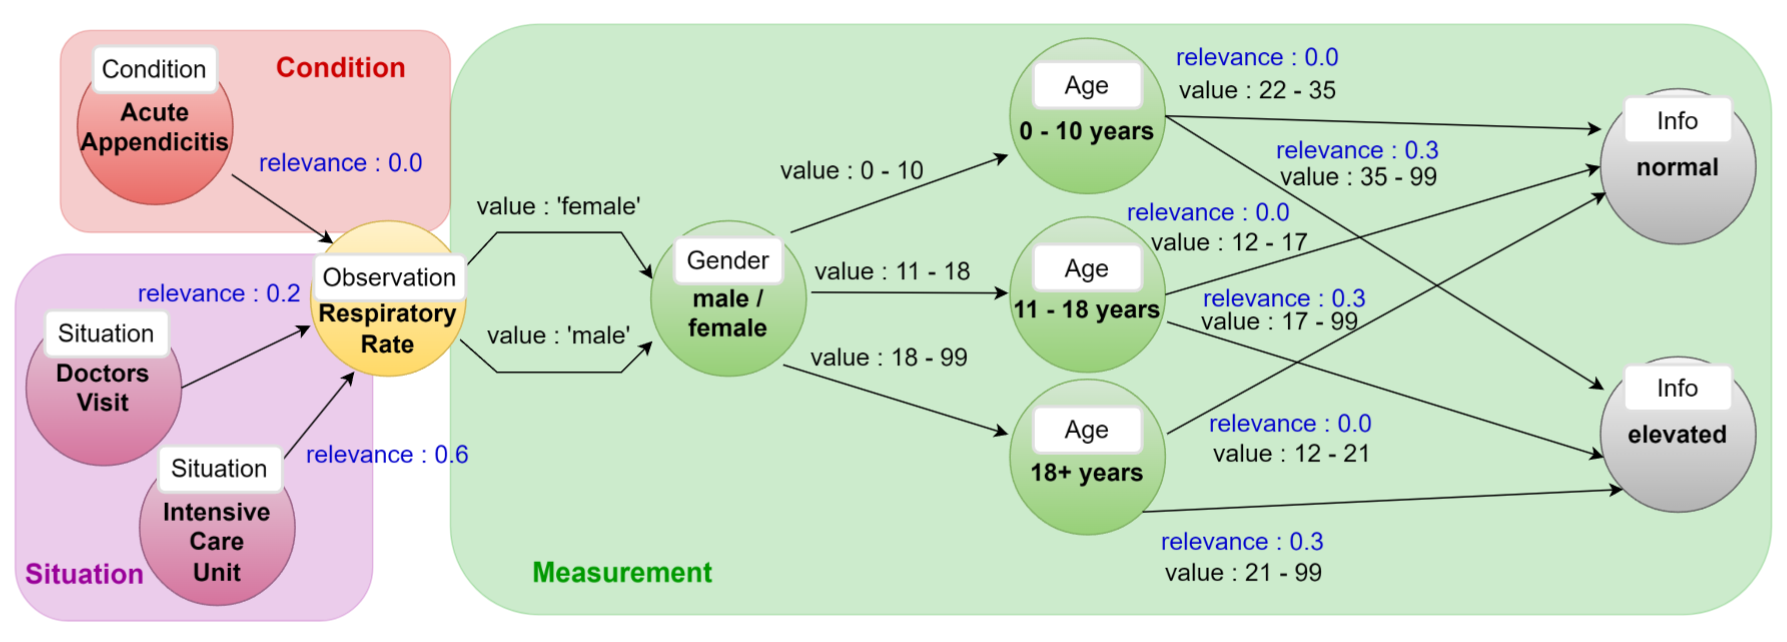
\includegraphics[width=\picturewidth]{graph_example.png}
  \caption{Example subgraph for the observation "Respiration Rate" in relation to the condition "Acute Appendicitis" from \citeauthor{TOM}'s Thesis\\ \cite[subsection 4.3.2]{TOM}}
  \label{fig:graphExample}
\end{figure}

In his master's thesis \cite{TOM}, \citeauthor{TOM} designed a knowledge graph structure that uses relational information between patient condition (i.e. medical diagnoses), patient observations (i.e. laboratory values, pain responses, etc.) and situations (i.e. treatment locations) to support medical personell in the diagnosis and treatment process, as seen in \cref{fig:graphExample}. By utilizing scores describing the strength of connection between current observations, conditions and situation, it calculates the relevance of every present observation based on how critical treatment of said observation is. This can then be used to sort and filter these observations for display for the medical professionals, thus expediting the treatment process. Furthermore, based on the same scores, additional condition diagnoses can be suggested based on the presence of connected observations. The knowledge graph can additionally give medication recommendations for existing conditions, taking into account patient allergies.
All these features build on verified medical knowledge, which has to be encoded into the knowledge graph.

\section{Large Language Models}

Large Language Models (LLMs) are a class of ML \cite{samuelStudiesMachineLearning1959} systems designed to process and generate natural language by training the model to predict the next token in a sequence \cite{wangHistoryDevelopmentPrinciples2025}. By training the model on very large corpora of raw text, a rich representation of language is aquired, that can be adapted to question answering, reasoning, or summarization through fine-tuning \cite{radfordImprovingLanguageUnderstanding2018}. 

, demonstrated how large-scale unsupervised training on raw text could yield models that generalize effectively across diverse downstream tasks. In this framework, the model is trained to predict the next token in a sequence, 

% In the broader sense, machine learning refers to computer programs that improve their performance on a given task through experience, rather than following explicitly hard-coded rules~\cite{samuel_ml}. LLMs instantiate this principle by learning statistical patterns of language from vast text corpora.
They are predominantly based on the \emph{Transformer} architecture \cite{vaswaniAttentionAllYou2023}, which introduced the attention mechanism as a means of modeling dependencies across an entire sequence of tokens, capturing long-range contextual relationships, a property essential for coherent language modeling over extended passages of text.

Current state-of-the-art proprietary LLMs include GPT-5 \cite{IntroducingGPT52025}, Gemini 2.0 \cite{IntroducingGemini202024} and Claude 4 \cite{IntroducingClaude4}. In the open-source domain, several models provide alternatives, including Llama 3.1 \cite{IntroducingLlama31,grattafioriLlama3Herd2024}, Gemma3 \cite{teamGemma3Technical2025}, Mistral \cite{jiangMistral7B2023}, Qwen \cite{baiQwenTechnicalReport2023} and BLOOM \cite{workshopBLOOM176BParameterOpenAccess2023}.

\section{Medical Information Extraction}
\label{sec:MedicalIE}

The domain of medical information extraction has seen a lot of development, with a plethora of human-designed and implemented methods utilizing rule-based approaches and utilizing natural language processing (NLP) machine learning technologies in named entity recognition, relation extraction, section detection and text indexing \cite{landolsiInformationExtractionElectronic2023}.

The introduction of deep learning (DL) models brought a new wave of development, with specialized deep learning models able to outperform feature engineered models in multiple IE fields \cite{hahnMedicalInformationExtraction2020}, including event extraction \cite{maDICEDataEfficientClinical2023} and entity relation extraction \cite{hussainAIDrivenKnowledge2020}.
% - Deep learning vs feature engineered models, medical texts, survey/shows that DL-models can outperform feature engineered approaches to information extraction tasks \cite{hahnMedicalInformationExtraction2020}
% - machine learning, medical texts, clinical event extraction \cite{maDICEDataEfficientClinical2023}
% - deep learning, MPGs, Entity relation extraction \cite{hussainAIDrivenKnowledge2020}

While in their base form still sometimes underperforming in certain IE fields relative to specialized models \cite{naguibFewshotClinicalEntity2024}, LLMs also show great promise. GPT-3 shows great zero- and one-shot performance in various clinical IE tasks \cite{agrawalLargeLanguageModels2022}. Other studies show that using fine-tuning allows a multitude of models to also excell in structured information extraction, for both high parameter count models (GPT-3 175B and Llama-2 70B \cite{dagdelenStructuredInformationExtraction2024}) as well as smaller models (PMC-Llama 13B, Llama-3-8B-UltraMedical, DeepSeek R1 distilled to Llama-3.1 8B, Qwen2.5-Math 7B, Llama-3.1 8B, Gemma-2-9B, and Mistral-v0.3 7B \cite{liuHumanlevelInformationExtraction2025}). The specially adapted and trained Llama2 variant VANER \cite{bianaVANERLeveragingLarge2024} also shows similar or higher performance in named entity recognition (NER) than traditional NER methods.

% - LLMs/machine learning/masked language models, clinical texts, clinical entity recognition \cite{naguibFewshotClinicalEntity2024}
% - GPT-3, medical texts, various NLP tasks \cite{agrawalLargeLanguageModels2022}
% - LLMs, scientific texts, structured information extraction \cite{dagdelenStructuredInformationExtraction2024}
% - !!!! LLMs, clinical notes, structured information extraction (with training) \cite{liuHumanlevelInformationExtraction2025}
% - LLMs, medical texts, named entity recognition \cite{bianaVANERLeveragingLarge2024}

With LLMs growing in popularity in the NLP field \cite{xiaAnalyzing16193LLM2025}, papers also focus in providing frameworks and pipelines for structured IE (RadEx \cites{reichenpfaderRadExFrameworkStructured2024},PLUMBER \cite{jaradehBetterCallPlumber2021a}), and named entity recognition (SKIPNER \cite{bianOneshotBiomedicalNamed2024}). LLMs are also used for prompt engineering to improve performance \cite{huImprovingLargeLanguage2024,zhangAutomaticPromptDesign2025} and generating fine-tuning data for specialized models \cite{meoniLargeLanguageModels2023}.
% - framework, radiology reports, structured information extraction \cite{reichenpfaderRadExFrameworkStructured2024}
% - !!!! LLMs, med text, clinical named entity recognition, prompt engineering \cite{huImprovingLargeLanguage2024}
% - LLMs, medical, automatic prompt design to improve information extraction \cite{zhangAutomaticPromptDesign2025}
% - machine learning, medical texts, using LLMs to generate fine-tuning data for specialized models \cite{meoniLargeLanguageModels2023}
% - LLMs, medical texts, named entity recognition in multipart pipeline approach \cite{bianOneshotBiomedicalNamed2024}
% - pipeline for information extraction tasks \cite{jaradehBetterCallPlumber2021a}

\section{Information Extraction Technologies for Medical Practice Guidelines}
\label{sec:IETecMPGs}

In the specific case of information extraction from MPGs, LLMs appear to not be used, with existing technologies relying on human made or traditional ML based approaches.

\citeauthor*{kaiserGainingProcessInformation2005} introduce a "multi-step transformation process" using intermediate representations of the MPGs by using heuristic methods to extract process information \cite{kaiserGainingProcessInformation2005}. They use a dictionary containing medical, action, condition relation and unit terms as well as special keywords to filter out irrelevant sentences and categorize the remaining sentences into annotation, process or negative action description. Furthermore, they use extracted sentence relation to form process relations. When evaluating their process on MPGs of otolaryngology, their approach achieves an average recall and precision in two tasks of $0.85$ and $0.91$ respectively.
% - human made, MPGs, information retrieval \cite{loglisciKnowledgeBasedFrameworkInformation2009}

\citeauthor*{loglisciKnowledgeBasedFrameworkInformation2009} developed an information extraction process of two phases \cite{loglisciKnowledgeBasedFrameworkInformation2009}. The first phase uses NLP functionalities to segment the MPG into sections, subsections and pieces of information, as well as extracting the semantics of the text into annotations. The second phase then uses a template structure based on medical decision problems, into which the annotated pieces of information are put, to transform any MPG into a uniform structure, while retaining relevant information. In an application to an "osteoporosis in gastrointestinal disease" MPG, this process achieved an average recall and precision of $0.85$ and $0.84$ in extracting three different decision problems.
% - human design/heuristics, MPGs, Process information \cite{kaiserGainingProcessInformation2005}

\citeauthor*{hussainTextClassificationClinical2021} introduce a process of creating patterns for MPG sentence classification into recommendation and non-recommmendation sentences \cite{hussainTextClassificationClinical2021}. ML algorithms are trained to extract salient terms for classification from a hypertension guideline, while a group of experts extracts initial classification patterns from the same guideline in three different forms, heuristic, part-of-speech(POS) and unified medical language system (UMLS). The salient terms are then provided to the experts to refine their patterns. When tested on MPGs on asthma, rhinosinusitis and hypertension, the combined patterns achieve a precision of $0.79$, $0.85$ and $0.92$ respectively.
% - Machine learning/human design, MPGs, Text classification with patterns \cite{hussainTextClassificationClinical2021}

\citeauthor*{fazlicNovelNLPFUZZYSystem2019} created a prototype system for fuzzy rule extraction \cite{fazlicNovelNLPFUZZYSystem2019}. A recurrent neural network with bi-directional long short-term memory was trained to annotate the MPG text with entity classes. These classes are then used by the "NLP-FUZZY system" to create fuzzy rules encoding recommendations included in the MPG, together with recommendation levels. In a validation process with 15 MPGs, this system achieved recall and precision of $0.84$ and $0.79$ with an $f1$-score of $0.81$, more than $0.1$ higher than other research models.
% - machine learning/human design, MPGs, information extraction \cite{fazlicNovelNLPFUZZYSystem2019}

% =================================================================================================
\chapter{Design}
\label{ch:Design}

To evaluate the LLMs selected in the section above on their reliability and correctness in extracting relevant data from MPGs, a prototype application for extracting this data is developed and run on a small set of prepared testing data, since no such testing dataset exists for this use case.

\section{Measurement Graph Structure}

\begin{figure}[h]
  \centering
  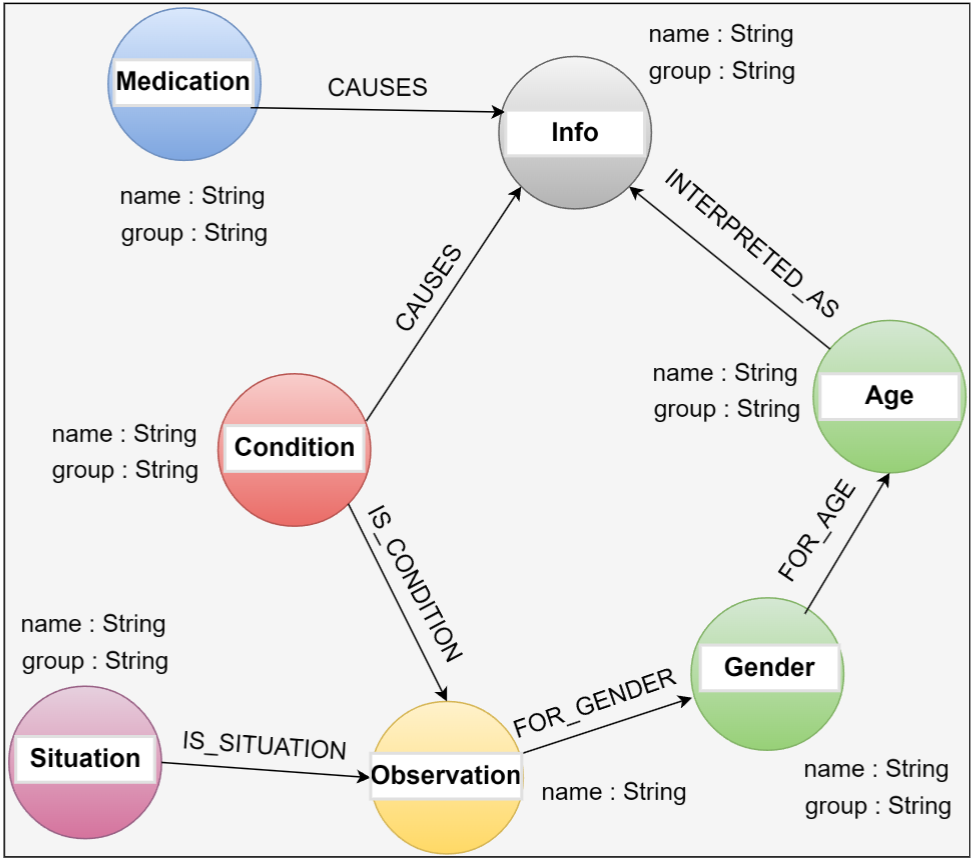
\includegraphics[width=\picturewidth]{measurement_graph_structure.png}
  \caption{Measurement Graph structure from \citeauthor{TOM}'s Thesis\\ \cite[subsection 4.4.1]{TOM}}
  \label{fig:graphStructure}
\end{figure}

The measurement graph structure, as illustrated in in \cref{fig:graphStructure}, encodes relationships between medications, conditions, observations, situations, and patient context (age and gender), with most of these connections encoding a relevance describing the strength of connection between nodes, as shown in \cref{fig:graphExample}.

The Observation nodes represents measurable findings about a patient. They are linked to Condition nodes, which encode different medical diagnoses, through an IS\_CONDITION relationship, capturing  how relevant each observation is to different diagnoses. Similarly, the Situation nodes, which represents contextual information such as whether the patient is in the ICU or at a routine check-up, are connected to observations through an IS\_SITUATION relationship, highlighting the importance to display said observation to the medical personell in this situation.

as described by \citeauthor{TOM}, the relevance of observations based on the observation measurement is encoded in the connection with Info nodes via INTERPRETED\_AS. These nodes provide interpretations for different measurement values. If this interpretation is dependent on patient demographic, the additional intermediate nodes Age and Gender can be introduced, allowing for nuanced differentiation. 

Additionally, certain conditions and medications can influence measurement values, which is encoded by connecting the Medication and Condition nodes with Info nodes, enabling the graph to capture how existing diagnoses and currently used medications can influence clinical interpretation of patient observations.

\section{Data Structure}

As the extracted data is intended to be used to extend the CAIS.ME KG, it should be provided in a \textit{data structure (DS)} similar to the structure of the KG, to make the extension process easier. \Citeauthor{loglisciKnowledgeBasedFrameworkInformation2009} suggests a handcrafted approach that uses template filling to enforce a specifically structured output. Following this line of thinking, the approach of this thesis utilizes a JSON schema representing the KG structure to support LLMs in extracting correctly formatted data containing the right relations between conditions, observations, situations and measurement interpretations.

Due to this thesis being a preliminary evaluation of LLM information extraction capability and limited computational capability, the \textit{DS} will only focus on the main part of this measurement graph structure, namely the nodes Observation, Condition, Situation, and Info. Furthermore, since this thesis does not aim to evaluate the LLMs capability of extracting factual information from the MPGs, the relevance scores between the nodes will not be taken into consideration. As \citeauthor{TOM} described in \cite[Section 7.2.2, Graph Generation]{TOM}, these relevance scores should follow specifically designed requirements and would be calculated over large datasets, which would be outside the scope of this evaluation.

With these restrictions, the \textit{DS} shown in \cref{fig:DataStructure} was designed based on the KG.

\begin{figure}[]
  \begin{minted}{python}
  class ConditionKnowledgeGraph:
    observations: List[Observation]
    conditions: List[Condition]

  class Condition:
    name: str
    observations: List[str]

  class Observation:
    name: str
    context: List[str]
    patient_inferences: List[PatientInference]

  class PatientInference:
    gender: Optional[Literal["female", "male", "nonbinary"]] = None
    age: Optional[PatientAge] = None
    inferences: List[Inference]

  class PatientAge:
    operator: Optional[Literal["<", "<=", "=", ">=", ">"]] = None
    value: Union[float, List[float]]
    unit: Literal["years", "months", "days"]

  class Inference:
    label: Optional[str]
    value_criterion: Optional[ValueCriterion] = None

  class ValueCriterion:
    operator: Optional[Literal["<", "<=", "=", ">=", ">", "approx"]] = None
    value: Union[float, List[float]] = None
    unit: str
  \end{minted}
  \caption{Representation of the \textit{DS} with python \textbf{pydantic} classes.}
  \label{fig:DataStructure}
\end{figure}

The \textit{DS} contains two lists, one holding observation information, and the other condition information. This decoupling of conditions and observations is due to them being in a many-to-many relationship. The condition objects only reference the related observations by name, and the exact observation information is contained in the observation objects.

Since the interpretations of patient observations are not always dependent on age or gender, as well as not always being exact value measurements, such as the presence of localized pain, the \textit{DS} makes these object attributes to be optional.

\begin{figure}[]
\begin{minted}{json}
  {
    "observations": [
      {
        "name": "<string>",
        "context": [
          "<list of string>"
        ],
        "patient_inferences": [
          {
            "gender": "<string>",
            "age": {
              "value": "<number or [number, number]>",
              "unit": "<string>",
              "operator": "<string>"
            }
            "inferences": [
              {
                "label": "<string>",
                "value_criterion": {
                  "value": "<number or [number, number]>",
                  "unit": "<string>",
                  "operator": "<string>"
                }
              }
            ]
          }
        ]
      }
    ],
  "conditions": [
    {
      "name": "<string>",
      "observations": [
        "<list of strings>"
      ]
    }
  ]
}
  \end{minted}
  \caption{Representation of \textit{DS} with a JSON schema.}
  \label{fig:JSONexample}
\end{figure}

The \textit{DS} allows for the representation of value ranges, either as an open ended range, such as "$>50$" or "$\le-0.5$", or an interval between two numbers, such as "$18-25$", since patient age and measurement values are mostly given in such value ranges. This is achieved by making the operator of such ranges optional, and giving the choice of either one or two values.

While the \textit{DS} was here implemented using the python \mintinline{python3}|pydantic| library, it can also be represented as a composition of lists and key-value based dictionaries as well as JSON code, with an example representation seen in \cref{fig:JSONexample}. Provided to the models will be a more nuanced schema, which encodes more structural information from the above class structure such as optional fields. This can be found in the appendix at \cref{fig:JSONschema}.

\section{Prompt Design}

To instruct the LLMs into extracting the correct information, a prompt is designed. The prompt is divided into four sections, task instruction, format instruction, example, and a final task instruction.
The first section contains a general explanation of the task, including an overview of the \textit{DS} and the instruction to output in the JSON format. The following section holds a JSON representation the \textit{DS}, as well as constrains for the representation of age and measurement values. As described in the previous section, in the \textit{DS}, value operators are optional and values can be given as one or two numbers. The prompt instructs the LLM to either put an operator and one value, representing the open value ranges, or no operator and two values, representing the intervals. The third section gives the model further restrictions on which information to put into the name and label attributes of the different objects and to only focus on direct patient observations and measurements. Finally, a small example is provided, and the guideline text is appended.
The finalized prompt can be seen in the appendix in \cref{sec:prompt}.

\section{Evaluation Algorithm}
\label{sec:EvalAlg}

To evaluate a models output compared to the expected \textit{ground truth}, the following process was designed.

First, the \textit{model output} is checked to be valid JSON code. If the \textit{model output} is invalid json code, it utilizes the \mintinline{python3}|pydantic_core.from_json()| function with \mintinline{python3}|allow_partial="on"|, thus receiving a now valid dictionary object, reflecting the \textit{DS} described above, containing the data extracted by the LLM.

The algorithm then evaluates how much correct and incorrect data the \textit{model output} contains by recursively traversing the \textit{model output} dictionary parallel to the \textit{ground truth} dictionary and calculating the amount of \textit{true\_positive}, \textit{false\_positive} and \textit{false\_negative} occurences of key value key value pairs of dictionaries. \textit{true\_positive} means in this setting, that the element in the \textit{ground truth} is correctly extracted in the \textit{model output}, while \textit{false\_positive} encompasses all generated data not related to the \textit{ground truth}, and \textit{false\_negative} contains all elements from the \textit{ground truth} that are not present in the \textit{model output}. 

When the values of \textit{model output} and \textit{ground truth} are the same type, the values are compared based on their similarity. If the values are text (strings), the comparison is based on string similarity calculated with the python \mintinline{python3}|SequenceMatcher.ratio()|\footnote{\citefield{DifflibHelpersComputing}{howpublished}}, with scores of $>0.6$ being regarded as true positive, while those below are regarded as not matching and as such both a false posisitive as well as a false negative. Numbers are directly compared, with same and different numbers being handled the same way as strings.
In the case of the value being a list, each pairing of elements from the \textit{ground truth} and \textit{model output} lists is scored recursively, and then the best matching is calculated using the modified Jonker-Volgenant algorithm \cite{crouseImplementing2DRectangular2016} with the python function \mintinline{python3}|scipy.optimize.linear_sum_assignment|\footnote{\href{https://docs.scipy.org/doc/scipy/reference/generated/scipy.optimize.linear_sum_assignment.html}{https://docs.scipy.org/doc/scipy/reference/generated/scipy.optimize.linear\_sum\_assignment.html}}. Similarly, if the value is a dictionary, its key value pairs are recursively compared.
If \textit{model output} elements could not be matched to any element in the \textit{ground truth}, they regarded as incorrect input. Similarly, \textit{ground truth} items which could not be matched to any output item are regarded as missed information. 

% =================================================================================================
\chapter{Evaluation}
\label{ch:Evaluation}

In the previous chapter, the parts necessary for extracting information were prepared. In this chapter the process of evaluating LLMs will be explained, with preparation of evaluation data, choosing which models to evaluate, and implementation of evaluation software.

\section{Evaluation Data}
\label{sec:EvaluationData}

To evaluate the models, a \textit{ground truth} with which to compare the outputs is created.
Two MPGs pertaining to the conditions of hypertension \cite{mcevoy2024ESCGuidelines2024} and acute appendicitis \cite{snyderAcuteAppendicitisEfficient2018} are chosen due to them being used as examples by \cite{TOM} when explaining the KG structure.
From these MPGs, small sections of text and tables are selected, which can be seen in the appendix under \cref{sec:guidelineText}.

Based on the \textit{DS} designed in the previous chapter, all relevant conditions, observations and situations are extracted by human hand (\cref{fig:GTHyp} and \cref{fig:GTAcu}). To examine this extracted data for correctness and relevance, it was transformed into an excel file (\cref{sec:excel}) and send to medical professionals, who approved the data as \textit{ground truth}.

\section{Implementation}

The evaluation is performed by utilizing Ollama \cite{Ollama},an open-source software for running open-source LLMs locally. This approach was chosen due to the simplicity of the interface to iterate different model parameters, which is necessary for evaluation of said parameters, as well as the ability to run many different models independent from cloud-based computing. With this a prototype program was developed containing an inference and an evaluation process.

The first process instructs specified LLMs to extract information from the selected MPG texts by providing the prompt designed in the previous chapter, the text, and the model parameters \temperature, \topP and \topK. The program also provides the JSON schema of the \textit{DS} directly to Ollama, as it also supports the ability to provide an output schema which the models will adhere to.
The program runs this extraction for each model once for each of the previously chosen MPGs with each combination of the parameters \temperature, \topP and \topK with the respective values $(0.0, 0.2, .., 1.0)$,$(0.0, 0.2, .., 1.0)$ and $(20,40,80)$, leading to a total of 108 evaluations per model.

To avoid the case of the model running into an endless loop, the number of tokens the models can predict is restricted by providing Ollama with the parameter $num\_predict = 3000$, which is more than enough tokens to output the target data.

The second process utilizes the evaluation algorithm described in \cref{sec:EvalAlg} to compares the models output for the amount of correctly and incorrectly extracted data with the \textit{ground truth} from the evaluation data described in \cref{sec:EvaluationData}. These results are then accumulated for each evaluated model, parameter and evaluation data. The code for this prototype implementation can be found on \url{https://github.com/darthdrannel/LLM_evaluation_thesis}.

\section{Model Selection}

With utilizing Ollama, the selection of models is restricted to those with public weights, i.e. open-source models, that are present in the Ollama database. From the list of possible LLMs, this thesis uses the following three different model architectures to test how different architecture influences output data correctness.
Due to the available local hardware, the model sizes used in the evaluation are restricted to models able to run on a single NVidia K80 GPU. This also limits the context window, the amount of previous tokens a model takes into account when generating more text, to $8000$, since larger context size increases the needed VRAM. This context window size is large enough to include the prompt, MPG text and any already model-infered tokens given the $3000$ token prediction limit.

\begin{itemize}
  \item Llama3.1-Instruct 8B\footnote{\citefield{Llama31}{howpublished}} \cite{grattafioriLlama3Herd2024}
  \item Mistral-Instruct-0.2 7B\footnote{\citefield{Mistral}{howpublished}} \cite{jiangMistral7B2023}
  \item Gemma3 4B\footnote{\citefield{Gemma3}{howpublished}} \cite{teamGemma3Technical2025}
\end{itemize}

To examine if using models fine-tuned for medical reasoning produce better outputs, for each model architecture a version fine-tuned on medical reasoning tasks is also used.

\begin{itemize}
  \item Llama3-Med42 (Llama3 8B Distillation of Med42)\footnote{\citefield{ThewindmomLlama3med428b}{howpublished}} \cite{christopheMed42v2SuiteClinical2024}
  \item LLaVA-Medv1.5-Mistral0.2 (Mistral0.2 7B Distillation of LLaVA-Med v1.5)\footnote{\citefield{ZuoLlavamedv15mistral7b_q8_0}{howpublished}} \cite{liLLaVAMedTrainingLarge2023}
  \item MedGemma 4B\footnote{\citefield{AlibayramMedgemma}{howpublished}} \cite{sellergrenMedGemmaTechnicalReport2025}
\end{itemize}

In addition to evaluating this collection of lightweight LLMs, a comparison with GPT-5 \cite{IntroducingGPT52025} is also included. While the exact architecture and parameterization of GPT-5 are not publicly disclosed, it currently represents the state-of-the-art in deployed LLM systems. Including GPT-5 in the evaluation provides a practical upper bound on performance, contextualizing the capabilities and limitations of smaller-scale models relative to a industry-leading system with orders of magnitude more computing power and parameters.

% =================================================================================================
\newpage
\section{Results}

This section describes the results of the evaluation while answering he questions posed in posed in the introduction.

\subsection{Data Structure Adherence}

\begin{table}[]
  \footnotesize
  \centering
  \begin{tabular}{|c|c||c|c|c|c|}
    \hline
    \textbf{Model Group} & \textbf{Model} & \multicolumn{2}{|c|}{\textbf{valid JSON}} & \multicolumn{2}{|c|}{\textbf{valid DS}$^*$}\\
    \hline\hline
    \multirow{2}{*}{Llama} & Llama3.1-Instruct & \multirow{2}{*}{\gettablepercentage{0}{vJSON}{\tableAvgModels}}& \gettablepercentage{3}{vJSON}{\tableAvgModels} & \multirow{2}{*}{\gettablepercentage{0}{vStruct}{\tableAvgModels}}& \gettablepercentage{3}{vStruct}{\tableAvgModels}\\
    \cline{2-2}\cline{4-4}\cline{6-6}
    & Llama3-Med42 & & \gettablepercentage{6}{vJSON}{\tableAvgModels} & & \gettablepercentage{6}{vStruct}{\tableAvgModels}\\
    \hline
    \multirow{2}{*}{Mistral} & Mistral-Instruct-0.2 & \multirow{2}{*}{\gettablepercentage{1}{vJSON}{\tableAvgModels}}& \gettablepercentage{4}{vJSON}{\tableAvgModels} & \multirow{2}{*}{\gettablepercentage{1}{vStruct}{\tableAvgModels}}& \gettablepercentage{4}{vStruct}{\tableAvgModels}\\
    \cline{2-2}\cline{4-4}\cline{6-6}
    & LLaVA-Medv1.5-Mistral0.2 & & \gettablepercentage{7}{vJSON}{\tableAvgModels} & & \gettablepercentage{7}{vStruct}{\tableAvgModels}\\
    \hline
    \multirow{2}{*}{Gemma} & Gemma3 & \multirow{2}{*}{\gettablepercentage{2}{vJSON}{\tableAvgModels}}& \gettablepercentage{5}{vJSON}{\tableAvgModels} & \multirow{2}{*}{\gettablepercentage{2}{vStruct}{\tableAvgModels}}& \gettablepercentage{5}{vStruct}{\tableAvgModels}\\
    \cline{2-2}\cline{4-4}\cline{6-6}
    & MedGemma & & \gettablepercentage{8}{vJSON}{\tableAvgModels} & & \gettablepercentage{8}{vStruct}{\tableAvgModels}\\
    \hline
  \end{tabular}
  \caption{Percentage of valid JSON output over all parameter configurations for each model architecture and evaluated Model\\$^*$\textit{\textit{DS}}}
  \label{table:DSModelStructure}
\end{table}

With the use of a token prediction limit, as mentioned in the implementation section, the possibility of incomplete output data is present. This limit is multiple times higher than the tokens needed to express the expected extracted information. Incomplete output data, i.e. an invalid/truncated JSON structure, thus indicates that the model encountered one of the following problems: creating vast amounts of incorrect data; repeating already extracted data; falling into an endless loop. These problems mean the model intends to output more than the allowed limit of $3000$ tokens, which means the intended JSON code is truncated, leading to invalid JSON.

% fig:validJSON
\begin{figure}[]
  \centering
  \begin{tikzpicture}
    \begin{axis}[
        xlabel = \temperature,
        ylabel = valid JSON output,
        yminorticks,
        yticklabel=\pgfmathparse{100*\tick}\pgfmathprintnumber{\pgfmathresult}\,\%,
        ymax = 1.0,
        minor y tick num = 1,
        ymajorgrids,
        yminorgrids,
        ymin=0.0,
        width=\graphwidth,
        ybar = 0pt,
        bar width = \barwidth,
        axis lines = left,
        enlarge y limits = 0.05,
        enlarge x limits = 0.15,
        legend style={font=\footnotesize},
        legend columns=3,
        legend entries={Llama3.1-Instruct, Mistral-Instruct-v0.2, Gemma3, Llama3-Med42, LLaVA-Med-1.5-Mistral, MedGemma},
        legend to name=graph:valid
      ]

      \addplot[CMap=\colorA]
      table[y=llamains_vJSON]{\tableAvgTemp};
      \addplot[CMap=\colorB]
      table[y=mistrins_vJSON]{\tableAvgTemp};
      \addplot[CMap=\colorC]
      table[y=gemma_vJSON]{\tableAvgTemp};
      \addplot[CMap=\colorD]
      table[y=llamamed_vJSON]{\tableAvgTemp};
      \addplot[CMap=\colorE]
      table[y=llavamed_vJSON]{\tableAvgTemp};
      \addplot[CMap=\colorF]
      table[y=medge_vJSON]{\tableAvgTemp};
      
      \coordinate (A) at (axis cs:1,\GPTvJSON);
      \coordinate (O1) at (rel axis cs:0,0);
      \coordinate (O2) at (rel axis cs:1,0);

      \draw [black,sharp plot, dashed] (A -| O1) -- (A -| O2);

    \end{axis}
  \end{tikzpicture}
  \hfill
  \begin{tikzpicture}
    \begin{axis}[
        xlabel = \topP,
        yticklabel=\empty,
        yminorticks,
        minor y tick num = 1,
        ymax = 1.0,
        ymajorgrids,
        yminorgrids,
        ymin=0.0,
        width=\graphwidth,
        ybar = 0pt,
        bar width = \barwidth,
        axis lines = left,
        enlarge y limits = 0.05,
        enlarge x limits = 0.15,
        legend style={font=\footnotesize, at={(0.5,1)}, anchor=south},
      ]
      
      \addlegendimage{line legend,black,sharp plot, dashed}
      \addlegendentry{GPT-5}

      \addplot[CMap=\colorA]
      table[y=llamains_vJSON]{\tableAvgTopP};
      \addplot[CMap=\colorB]
      table[y=mistrins_vJSON]{\tableAvgTopP};
      \addplot[CMap=\colorC]
      table[y=gemma_vJSON]{\tableAvgTopP};
      \addplot[CMap=\colorD]
      table[y=llamamed_vJSON]{\tableAvgTopP};
      \addplot[CMap=\colorE]
      table[y=llavamed_vJSON]{\tableAvgTopP};
      \addplot[CMap=\colorF]
      table[y=medge_vJSON]{\tableAvgTopP};
 
      \coordinate (A) at (axis cs:1,\GPTvJSON);
      \coordinate (O1) at (rel axis cs:0,0);
      \coordinate (O2) at (rel axis cs:1,0);

      \draw [black,sharp plot, dashed] (A -| O1) -- (A -| O2);

    \end{axis}
  \end{tikzpicture}
  \hfill
  \begin{tikzpicture}
    \begin{axis}[
        xlabel = \topK,
        yticklabel=\empty,
        minor y tick num = 1,
        ymax = 1.0,
        ymajorgrids,
        yminorticks,
        yminorgrids,
        ymin=0.0,
        width=\graphwidth,
        ybar = 0pt,
        bar width = \barwidth,
        axis lines = left,
        enlarge y limits = 0.05,
        enlarge x limits = 0.15,
        symbolic x coords = {20,40,80},
      ]

      \addplot[CMap=\colorA]
      table[y=llamains_vJSON]{\tableAvgTopK};
      \addplot[CMap=\colorB]
      table[y=mistrins_vJSON]{\tableAvgTopK};
      \addplot[CMap=\colorC]
      table[y=gemma_vJSON]{\tableAvgTopK};
      \addplot[CMap=\colorD]
      table[y=llamamed_vJSON]{\tableAvgTopK};
      \addplot[CMap=\colorE]
      table[y=llavamed_vJSON]{\tableAvgTopK};
      \addplot[CMap=\colorF]
      table[y=medge_vJSON]{\tableAvgTopK};

      \coordinate (A) at (axis cs:20,\GPTvJSON);
      \coordinate (O1) at (rel axis cs:0,0);
      \coordinate (O2) at (rel axis cs:1,0);

      \draw [black,sharp plot, dashed] (A -| O1) -- (A -| O2);

    \end{axis}
  \end{tikzpicture}
  \\
  \ref{graph:valid}
  \caption{Percentage of valid JSON output from model with $max\_new\_tokens = 3000$ depending on parameters \temperature, \topP and \topK}
  \label{fig:validJSON}
\end{figure}

\cref{table:DSModelStructure} displays the percentage of model parameter configurations which have lead to the \textit{model output} being valid JSON code. This highlights that model architecture can influence the ability to produce valid JSON. The Llama based models display the highest performance of \gettablepercentage{0}{vJSON}{\tableAvgModels}, with Mistral based models coming close with a drop in about $10$ percentage points, and Gemma based models clearly underperforming with only \gettablepercentage{2}{vJSON}{\tableAvgModels}. This suggests that different model architectures are more suceptible to changes in parameters leading to encountering one of the problems mentioned above.

% fig:validDS
\begin{figure}[]
  \centering
  \begin{tikzpicture}
    \begin{axis}[
        xlabel = \temperature,
        ylabel = valid \textit{DS},
        yticklabel=\pgfmathparse{100*\tick}\pgfmathprintnumber{\pgfmathresult}\,\%,
        ymax = 1.0,
        ymajorgrids,
        yminorticks,
        minor y tick num = 1,
        yminorgrids,
        ymin=0.0,
        width=\graphwidth,
        ybar = 0pt,
        bar width = \barwidth,
        axis lines = left,
        enlarge y limits = 0.05,
        enlarge x limits = 0.15,
      ]
      \addplot[CMap=\colorA]
      table[y=llamains_vStruct]{\tableAvgTemp};
      \addplot[CMap=\colorB]
      table[y=mistrins_vStruct]{\tableAvgTemp};
      \addplot[CMap=\colorC]
      table[y=gemma_vStruct]{\tableAvgTemp};
      \addplot[CMap=\colorD]
      table[y=llamamed_vStruct]{\tableAvgTemp};
      \addplot[CMap=\colorE]
      table[y=llavamed_vStruct]{\tableAvgTemp};
      \addplot[CMap=\colorF]
      table[y=medge_vStruct]{\tableAvgTemp};

            
      \coordinate (A) at (axis cs:1,\GPTvStruct);
      \coordinate (O1) at (rel axis cs:0,0);
      \coordinate (O2) at (rel axis cs:1,0);

      \draw [black,sharp plot, dashed] (A -| O1) -- (A -| O2);
    \end{axis}
  \end{tikzpicture}
  \hfill
  \begin{tikzpicture}
    \begin{axis}[
        xlabel = \topP,
        yticklabel=\empty,
        ymax = 1.0,
        ymajorgrids,
        yminorticks,
        minor y tick num = 1,
        yminorgrids,
        ymin=0.0,
        width=\graphwidth,
        ybar = 0pt,
        bar width = \barwidth,
        axis lines = left,
        enlarge y limits = 0.05,
        enlarge x limits = 0.15,
        xtick = data,
        legend style={font=\footnotesize, at={(0.5,1)}, anchor=south},
      ]
      
      \addlegendimage{line legend,black,sharp plot, dashed}
      \addlegendentry{GPT-5}

      \addplot[CMap=\colorA]
      table[y=llamains_vStruct]{\tableAvgTopP};
      \addplot[CMap=\colorB]
      table[y=mistrins_vStruct]{\tableAvgTopP};
      \addplot[CMap=\colorC]
      table[y=gemma_vStruct]{\tableAvgTopP};
      \addplot[CMap=\colorD]
      table[y=llamamed_vStruct]{\tableAvgTopP};
      \addplot[CMap=\colorE]
      table[y=llavamed_vStruct]{\tableAvgTopP};
      \addplot[CMap=\colorF]
      table[y=medge_vStruct]{\tableAvgTopP};

            
      \coordinate (A) at (axis cs:1,\GPTvStruct);
      \coordinate (O1) at (rel axis cs:0,0);
      \coordinate (O2) at (rel axis cs:1,0);

      \draw [black,sharp plot, dashed] (A -| O1) -- (A -| O2);

    \end{axis}
  \end{tikzpicture}
  \hfill
  \begin{tikzpicture}
    \begin{axis}[
        xlabel = \topK,
        yticklabel=\empty,
        ymax = 1.0,
        ymajorgrids,
        yminorticks,
        minor y tick num = 1,
        yminorgrids,
        ymin=0.0,
        width=\graphwidth,
        ybar = 0pt,
        bar width = \barwidth,
        axis lines = left,
        enlarge y limits = 0.05,
        enlarge x limits = 0.15,
        symbolic x coords = {20,40,80},
        xtick = data,
      ]

      \addplot[CMap=\colorA]
      table[y=llamains_vStruct]{\tableAvgTopK};
      \addplot[CMap=\colorB]
      table[y=mistrins_vStruct]{\tableAvgTopK};
      \addplot[CMap=\colorC]
      table[y=gemma_vStruct]{\tableAvgTopK};
      \addplot[CMap=\colorD]
      table[y=llamamed_vStruct]{\tableAvgTopK};
      \addplot[CMap=\colorE]
      table[y=llavamed_vStruct]{\tableAvgTopK};
      \addplot[CMap=\colorF]
      table[y=medge_vStruct]{\tableAvgTopK};

      \coordinate (A) at (axis cs:20,\GPTvStruct);
      \coordinate (O1) at (rel axis cs:0,0);
      \coordinate (O2) at (rel axis cs:1,0);

      \draw [black,sharp plot, dashed] (A -| O1) -- (A -| O2);

    \end{axis}
  \end{tikzpicture}
  \\
  \ref{graph:valid}
  \caption{Percentage output being valid \textit{DS} with $max\_new\_tokens = 3000$ depending on parameters \temperature, \topP and \topK}
  \label{fig:validDS}
\end{figure}

Also noticeable in \cref{table:DSModelStructure} is that fine-tuning a model for medical question answering \textit{can} also lead to being more suceptiple of encountering one of the output problems. While Llama3-Med42 \cite{christopheMed42v2SuiteClinical2024} is slightly better than Llama3.1-Instruct \cite{grattafioriLlama3Herd2024}, both LLaVA-Medv1.5-Mistral0.2 \cite{liLLaVAMedTrainingLarge2023} and MedGemma \cite{sellergrenMedGemmaTechnicalReport2025} clearly underperform in relation to their parent models.

\cref{fig:validJSON} shows that model parameters do not influence the percentage of valid JSON output in a meaningful way. The small variations shown in \cref{fig:validJSON} can be explained by the inherent randomness of LLMs and the small sample size.

As expressed in \cref{fig:validDS} and \cref{table:DSModelStructure}, the evaluated model's output follows the \textit{DS} with almost the same percentages as it being a valid JSON string. This is caused by the models creating vast amounts of data, related to the list of observations in the \textit{DS}, or repeating single token groups indefinetly, thus being cut off by the token prediction limit before being able to extract any conditions. As the conditions list is a required field of the \textit{DS}, these outputs are considered invalid.

\pgfplotstablegetelem{5}{vStruct}\of{\tableAvgModels}
\edef\GvS{\pgfplotsretval}
\pgfplotstablegetelem{5}{vJSON}\of{\tableAvgModels}
\edef\GvJ{\pgfplotsretval}
\pgfmathparse{(\GvS - \GvJ) / (1 - \GvJ)}
\edef\Gval{\pgfmathresult}

\pgfplotstablegetelem{8}{vStruct}\of{\tableAvgModels}
\edef\MGvS{\pgfplotsretval}
\pgfplotstablegetelem{8}{vJSON}\of{\tableAvgModels}
\edef\MGvJ{\pgfplotsretval}
\pgfmathparse{(\MGvS - \MGvJ) / (1 - \MGvJ)}
\edef\MGval{\pgfmathresult}

The exceptions are Gemma3 with \percentage[round-precision=1]{\Gval} and MedGemma with \percentage[round-precision=1]{\MGval} of their invalid JSON outputs still conforming by the \textit{DS}. This anomaly can be explained by Gemma3 in a few cases not extracting any observations at all, thus resulting in an empty list, followed by the conditions list containing a endlessly repeating character sequence. MedGemma however often extracts plenty of duplicate data, thus almost filling the token limit with observation extractions, resulting in the condition list being present, but truncated.

% fig:boxplotModels
\begin{figure}[]
  \centering
  \begin{tikzpicture}
    \begin{axis}[
        ylabel = \textit{precision},
        width=\Graphwidth,
        height=\Graphheight,
        cycle list name= colorlist,
        boxplot/draw direction=y,
        xtick=\empty,
        ymax=0.75,ytick={0,0.25,0.5,0.75},minor y tick num = 1,yminorgrids,
        ymajorgrids,
        axis lines=left,
        enlarge y limits = 0.05,
        enlarge x limits = 0.05,
        legend style={font=\footnotesize, at={(1,1)}, anchor=north east},
      ]

      
      \addlegendimage{line legend,black,sharp plot, dashed}
      \addlegendentry{GPT-5}

      \pgfplotstablegetrowsof{\tablePreModels}
      \pgfmathtruncatemacro\TotalRows{\pgfplotsretval-1}
      \pgfplotsinvokeforeach{3,...,\TotalRows}
      {
        \addplot+[
          boxplot prepared from table={
            table=\tablePreModels,
            row=#1,
            lower whisker=lw,
            upper whisker=uw,
            lower quartile=lq,
            upper quartile=uq,
            median=med,
            draw position=pos,
            average=avg
          },
          boxplot prepared, fill=.!70!white, draw=.!50!black,
        ]
        coordinates {};
      }
      
      \coordinate (A) at (axis cs:1,\GPTPre);
      \coordinate (O1) at (rel axis cs:0,0);
      \coordinate (O2) at (rel axis cs:1,0);

      \draw [black,sharp plot, dashed] (A -| O1) -- (A -| O2);

    \end{axis}
  \end{tikzpicture}
  \begin{tikzpicture}
    \begin{axis}[
        ylabel = \textit{recall},
        width=\Graphwidth,
        height=\Graphheight,
        cycle list name = colorlist,
        boxplot/draw direction=y,
        xtick=\empty,
        ymax=0.75,ytick={0,0.25,0.5,0.75},minor y tick num = 1,yminorgrids,
        ymajorgrids,
        axis lines=left,
        enlarge y limits = 0.05,
        enlarge x limits = 0.05,
        legend columns=3,
        legend style={font=\footnotesize},
        legend entries={Llama3.1-Instruct, Mistral-Instruct-v0.2, Gemma3, Llama3-Med42, LLaVA-Med-1.5-Mistral, MedGemma},
        legend to name=graph:boxplot,
      ]
      

      \pgfplotstablegetrowsof{\tableRecModels}
      \pgfmathtruncatemacro\TotalRows{\pgfplotsretval-1}
      \pgfplotsinvokeforeach{3,...,\TotalRows}
      {
        \addplot+[
          boxplot prepared from table={
            table=\tableRecModels,
            row=#1,
            lower whisker=lw,
            upper whisker=uw,
            lower quartile=lq,
            upper quartile=uq,
            median=med,
            draw position=pos,
            average=avg,
          },
          boxplot prepared,
          fill=.!70!white,
          draw=.!50!black,
          area legend
        ]
        coordinates {};
      }

      
      \coordinate (A) at (axis cs:1,\GPTRec);
      \coordinate (O1) at (rel axis cs:0,0);
      \coordinate (O2) at (rel axis cs:1,0);

      \draw [black,sharp plot, dashed] (A -| O1) -- (A -| O2);

    \end{axis}
  \end{tikzpicture}
  \\
  \ref{graph:boxplot}
  \caption{Precision and recall distributions for the different models, aggregated over all combinations of \temperature, \topP and \topK.}
  \label{fig:boxplotModels}
\end{figure}


\subsection{Data Correctness}

%table:prerecModels
\begin{table}[]
  \footnotesize
  \centering
  \sisetup{table-alignment-mode = none} %table-format = 2.4, 
  \begin{tabular}{ c || c | c | c | >{\centering\arraybackslash}p{1.5cm} }
    \textbf{Model} & \textbf{\temp} & \textbf{\topP} & \textbf{\topK} & \textbf{\textit{precision}}\\
    \hline\hline
    Llama3.1-Instruct & \gettablefloat{1}{0}{temp}{\tableBestPre}& \gettablefloat{1}{0}{top_p}{\tableBestPre}& \gettablefloat{0}{0}{top_k}{\tableBestPre}& \textbf{\gettablefloat{3}{0}{value}{\tableBestPre}}
    \\
    Llama3-Med42 & \gettablefloat{1}{3}{temp}{\tableBestPre}& \gettablefloat{1}{3}{top_p}{\tableBestPre}& \gettablefloat{0}{3}{top_k}{\tableBestPre}& \gettablefloat{3}{3}{value}{\tableBestPre}
    \\
    \hline
    Mistral-Instruct-0.2 & \gettablefloat{1}{1}{temp}{\tableBestPre}& \gettablefloat{1}{1}{top_p}{\tableBestPre}& \gettablefloat{0}{1}{top_k}{\tableBestPre}& \gettablefloat{3}{1}{value}{\tableBestPre}
    \\
    LLaVA-Medv1.5-Mistral0.2 & \gettablefloat{1}{4}{temp}{\tableBestPre}& \gettablefloat{1}{4}{top_p}{\tableBestPre}& \gettablefloat{0}{4}{top_k}{\tableBestPre}& \gettablefloat{3}{4}{value}{\tableBestPre}
    \\
    \hline
    Gemma3 & \gettablefloat{1}{2}{temp}{\tableBestPre}& \gettablefloat{1}{2}{top_p}{\tableBestPre}& \gettablefloat{0}{2}{top_k}{\tableBestPre}& \gettablefloat{3}{2}{value}{\tableBestPre}
    \\
    MedGemma & \gettablefloat{1}{5}{temp}{\tableBestPre}& \gettablefloat{1}{5}{top_p}{\tableBestPre}& \gettablefloat{0}{5}{top_k}{\tableBestPre}& \gettablefloat{3}{5}{value}{\tableBestPre}\\
    \hline\hline
    GPT-5 & \multicolumn{3}{|c|}{} & \num[round-mode = places,round-precision=3]{\GPTPre}
  \end{tabular}
  \\\vspace{3em}\hfill\\
  \begin{tabular}{c||c|c|c|>{\centering\arraybackslash}p{1.5cm}}
    \textbf{Model} & \textbf{\temp} & \textbf{\topP} & \textbf{\topK} & \textbf{\textit{recall}}\\
    \hline\hline
    Llama3.1-Instruct & \gettablefloat{1}{0}{temp}{\tableBestRec}& \gettablefloat{1}{0}{top_p}{\tableBestRec}& \gettablefloat{0}{0}{top_k}{\tableBestRec}& \textbf{\gettablefloat{3}{0}{value}{\tableBestRec}}\\
    Llama3-Med42 & \gettablefloat{1}{3}{temp}{\tableBestRec}& \gettablefloat{1}{3}{top_p}{\tableBestRec}& \gettablefloat{0}{3}{top_k}{\tableBestRec}& \gettablefloat{3}{3}{value}{\tableBestRec}\\
    \hline
    Mistral-Instruct-0.2 & \gettablefloat{1}{1}{temp}{\tableBestRec}& \gettablefloat{1}{1}{top_p}{\tableBestRec}& \gettablefloat{0}{1}{top_k}{\tableBestRec}& \textbf{\gettablefloat{3}{1}{value}{\tableBestRec}}\\
    LLaVA-Medv1.5-Mistral0.2 & \gettablefloat{1}{4}{temp}{\tableBestRec}& \gettablefloat{1}{4}{top_p}{\tableBestRec}& \gettablefloat{0}{4}{top_k}{\tableBestRec}& \gettablefloat{3}{4}{value}{\tableBestRec}\\
    \hline
    Gemma3 & \gettablefloat{1}{2}{temp}{\tableBestRec}& \gettablefloat{1}{2}{top_p}{\tableBestRec}& \gettablefloat{0}{2}{top_k}{\tableBestRec}& \gettablefloat{3}{2}{value}{\tableBestRec}\\
    MedGemma & \gettablefloat{1}{5}{temp}{\tableBestRec}& \gettablefloat{1}{5}{top_p}{\tableBestRec}& \gettablefloat{0}{5}{top_k}{\tableBestRec}& \gettablefloat{3}{5}{value}{\tableBestRec}\\
    \hline\hline
    GPT-5 & \multicolumn{3}{|c|}{} & \num[round-mode = places,round-precision=3]{\GPTRec}
  \end{tabular}
  \\\vspace{3em}\hfill\\
  \begin{tabular}{c||c|c|c|>{\centering\arraybackslash}p{1.5cm}}
    \textbf{Model} & \textbf{\temp} & \textbf{\topP} & \textbf{\topK} & \textbf{\textit{f1}}\\
    \hline\hline
    Llama3.1-Instruct & \gettablefloat{1}{0}{temp}{\tableBestFI}& \gettablefloat{1}{0}{top_p}{\tableBestFI}& \gettablefloat{0}{0}{top_k}{\tableBestFI}& \textbf{\gettablefloat{3}{0}{value}{\tableBestFI}}\\
    Llama3-Med42 & \gettablefloat{1}{3}{temp}{\tableBestFI}& \gettablefloat{1}{3}{top_p}{\tableBestFI}& \gettablefloat{0}{3}{top_k}{\tableBestFI}& \gettablefloat{3}{3}{value}{\tableBestFI}\\
    \hline
    Mistral-Instruct-0.2 & \gettablefloat{1}{1}{temp}{\tableBestFI}& \gettablefloat{1}{1}{top_p}{\tableBestFI}& \gettablefloat{0}{1}{top_k}{\tableBestFI}& \gettablefloat{3}{1}{value}{\tableBestFI}\\
    LLaVA-Medv1.5-Mistral0.2 & \gettablefloat{1}{4}{temp}{\tableBestFI}& \gettablefloat{1}{4}{top_p}{\tableBestFI}& \gettablefloat{0}{4}{top_k}{\tableBestFI}& \gettablefloat{3}{4}{value}{\tableBestFI}\\
    \hline
    Gemma3 & \gettablefloat{1}{2}{temp}{\tableBestFI}& \gettablefloat{1}{2}{top_p}{\tableBestFI}& \gettablefloat{0}{2}{top_k}{\tableBestFI}& \gettablefloat{3}{2}{value}{\tableBestFI}\\
    MedGemma & \gettablefloat{1}{5}{temp}{\tableBestFI}& \gettablefloat{1}{5}{top_p}{\tableBestFI}& \gettablefloat{0}{5}{top_k}{\tableBestFI}& \gettablefloat{3}{5}{value}{\tableBestFI}\\
    \hline\hline
    GPT-5 & \multicolumn{3}{|c|}{} & \num[round-mode = places,round-precision=3]{\GPTFI}
  \end{tabular}
  \caption{Parameter combinations for best \textit{precision}, \textit{recall} and \textit{f1} per model.}
  \label{table:prerecModels}
\end{table}

With the values from the evaluation for \textit{true\_positive}, \textit{false\_positive} and \textit{false\_negative} occurences of extracted information in the \textit{model output}, precision and recall values are calculated.

\cref{fig:boxplotModels} compares the precision and recall distributions of the evaluated models. Across all architectures, the general-purpose models (Llama3.1-Instruct, Mistral-Instruct-v0.2, and Gemma3) consistently achieve higher precision and recall than their medically fine-tuned counterparts (Llama3-Med42, LLaVA-Med-1.5-Mistral, and MedGemma), indicating that fine-tuning for medical question answering reduces precision and recall. Comparing across model architectures, Llama models show the strongest precision, while Mistral models achieve relatively balanced precision and recall. Gemma models lag behind in both metrics, with MedGemma's recall distribution appearing inflated due to often generating duplicate data, a problem mentioned above. These results suggest that model architecture plays a substantial role in determining output quality, with Llama and Mistral offering more reliable performance than Gemma in this setting.

% fig:boxplotParams
\begin{figure}[]
  \centering
  \ref{graph:boxplot}\\
  \begin{tikzpicture}
    \begin{axis}[
        xlabel = \temperature,
        ylabel = \textit{precision},
        width=\Graphwidth,
        height=\Graphheight,
        cycle list name= colorlist,
        boxplot/draw direction=y,
        xtick={3.5,12.5,...,48.5},
        xticklabels={0.0, 0.2, 0.4, 0.6, 0.8, 1.0},
        ymax=0.75,ytick={0,0.25,0.5,0.75},minor y tick num = 1,yminorgrids,
        ymajorgrids,
        axis lines=left,
        enlarge y limits = 0.05,
        enlarge x limits = 0.05,
        legend style={font=\footnotesize, at={(1,1)}, anchor=north east},
      ]
      
      % \addlegendimage{line legend,black,sharp plot, dashed}
      % \addlegendentry{GPT-5}

      \pgfplotstablegetrowsof{\tablePreTemp}
      \pgfmathtruncatemacro\TotalRows{\pgfplotsretval-1}
      \pgfplotsinvokeforeach{0,...,\TotalRows}
      {
        \addplot+[
          boxplot prepared from table={
            table=\tablePreTemp,
            row=#1,
            lower whisker=lw,
            upper whisker=uw,
            lower quartile=lq,
            upper quartile=uq,
            median=med,
            draw position=pos,
            average=avg
          },
          boxplot prepared, fill=.!70!white, draw=.!50!black,
          area legend
        ]
        coordinates {};
      }

      \coordinate (A) at (axis cs:1,\GPTPre);
      \coordinate (O1) at (rel axis cs:0,0);
      \coordinate (O2) at (rel axis cs:1,0);

      \draw [black,sharp plot, dashed] (A -| O1) -- (A -| O2);

    \end{axis}
  \end{tikzpicture}
  \begin{tikzpicture}
    \begin{axis}[
        xlabel = \temperature,
        ylabel = \textit{recall},
        width=\Graphwidth,
        height=\Graphheight,
        cycle list name = colorlist,
        boxplot/draw direction=y,
        xtick={3.5,12.5,...,48.5},
        xticklabels={0.0, 0.2, 0.4, 0.6, 0.8, 1.0},
        ymax=0.75,ytick={0,0.25,0.5,0.75},minor y tick num = 1,yminorgrids,
        ymajorgrids,
        axis lines=left,
        enlarge y limits = 0.05,
        enlarge x limits = 0.05,
      ]

      \pgfplotstablegetrowsof{\tableRecTemp}
      \pgfmathtruncatemacro\TotalRows{\pgfplotsretval-1}
      \pgfplotsinvokeforeach{0,...,\TotalRows}
      {
        \addplot+[
          boxplot prepared from table={
            table=\tableRecTemp,
            row=#1,
            lower whisker=lw,
            upper whisker=uw,
            lower quartile=lq,
            upper quartile=uq,
            median=med,
            draw position=pos,
            average=avg,
          },
          boxplot prepared,
          fill=.!70!white,
          draw=.!50!black,
        ]
        coordinates {};
      }

      \coordinate (A) at (axis cs:1,\GPTRec);
      \coordinate (O1) at (rel axis cs:0,0);
      \coordinate (O2) at (rel axis cs:1,0);

      \draw [black,sharp plot, dashed] (A -| O1) -- (A -| O2);

    \end{axis}
  \end{tikzpicture}
  \\
  \ref{graph:ChatGPT}\\
  \begin{tikzpicture}
    \begin{axis}[
        xlabel = \topP,
        ylabel = \textit{precision},
        width=\Graphwidth,
        height=\Graphheight,
        cycle list name = colorlist,
        boxplot/draw direction=y,
        xtick={3.5,12.5,...,48.5},
        xticklabels={0.0, 0.2, 0.4, 0.6, 0.8, 1.0},
        ymax=0.75,ytick={0,0.25,0.5,0.75},minor y tick num = 1,yminorgrids,
        ymajorgrids,
        axis lines=left,
        enlarge y limits = 0.05,
        enlarge x limits = 0.05,
        legend style={font=\footnotesize, at={(0.9,1)}, anchor=south},
        legend to name=graph:ChatGPT
      ]
      
      \addlegendimage{line legend,black,sharp plot, dashed}
      \addlegendentry{GPT-5}

      \pgfplotstablegetrowsof{\tablePreTopP}
      \pgfmathtruncatemacro\TotalRows{\pgfplotsretval-1}
      \pgfplotsinvokeforeach{0,...,\TotalRows}
      {
        \addplot+[
          boxplot prepared from table={
            table=\tablePreTopP,
            row=#1,
            lower whisker=lw,
            upper whisker=uw,
            lower quartile=lq,
            upper quartile=uq,
            median=med,
            draw position=pos,
            average=avg
          },
          boxplot prepared, fill=.!70!white, draw=.!50!black,
          area legend
        ]
        coordinates {};
      }
      \coordinate (A) at (axis cs:1,\GPTPre);
      \coordinate (O1) at (rel axis cs:0,0);
      \coordinate (O2) at (rel axis cs:1,0);

      \draw [black,sharp plot, dashed] (A -| O1) -- (A -| O2);
    \end{axis}
  \end{tikzpicture}
  \begin{tikzpicture}
    \begin{axis}[
        xlabel = \topP,
        ylabel = \textit{recall},
        width=\Graphwidth,
        height=\Graphheight,
        cycle list name = colorlist,
        boxplot/draw direction=y,
        xtick={3.5,12.5,...,48.5},
        xticklabels={0.0, 0.2, 0.4, 0.6, 0.8, 1.0},
        ymax=0.75,ytick={0,0.25,0.5,0.75},minor y tick num = 1,yminorgrids,
        ymajorgrids,
        axis lines=left,
        enlarge y limits = 0.05,
        enlarge x limits = 0.05,
      ]

      \pgfplotstablegetrowsof{\tableRecTopP}
      \pgfmathtruncatemacro\TotalRows{\pgfplotsretval-1}
      \pgfplotsinvokeforeach{0,...,\TotalRows}
      {
        \addplot+[
          boxplot prepared from table={
            table=\tableRecTopP,
            row=#1,
            lower whisker=lw,
            upper whisker=uw,
            lower quartile=lq,
            upper quartile=uq,
            median=med,
            draw position=pos,
            average=avg
          },
          boxplot prepared, fill=.!70!white, draw=.!50!black,
          area legend
        ]
        coordinates {};
      }

      \coordinate (A) at (axis cs:1,\GPTRec);
      \coordinate (O1) at (rel axis cs:0,0);
      \coordinate (O2) at (rel axis cs:1,0);

      \draw [black,sharp plot, dashed] (A -| O1) -- (A -| O2);

    \end{axis}
  \end{tikzpicture}
  \\
  \begin{tikzpicture}
    \begin{axis}[
        xlabel = \topK,
        ylabel = \textit{precision},
        width=\Graphwidth,
        height=\Graphheight,
        cycle list name = colorlist,
        boxplot/draw direction=y,
        xtick={3.5,12.5,...,48.5},
        xticklabels={0.0, 0.2, 0.4, 0.6, 0.8, 1.0},
        ymax=0.75,ytick={0,0.25,0.5,0.75},minor y tick num = 1,yminorgrids,
        ymajorgrids,
        axis lines=left,
        enlarge y limits = 0.05,
        enlarge x limits = 0.05,
      ]
      \pgfplotstablegetrowsof{\tablePreTopK}
      \pgfmathtruncatemacro\TotalRows{\pgfplotsretval-1}
      \pgfplotsinvokeforeach{0,...,\TotalRows}
      {
        \addplot+[
          boxplot prepared from table={
            table=\tablePreTopK,
            row=#1,
            lower whisker=lw,
            upper whisker=uw,
            lower quartile=lq,
            upper quartile=uq,
            median=med,
            draw position=pos,
            average=avg
          },
          boxplot prepared, fill=.!70!white, draw=.!50!black,
          area legend
        ]
        coordinates {};
      }

      \coordinate (A) at (axis cs:1,\GPTPre);
      \coordinate (O1) at (rel axis cs:0,0);
      \coordinate (O2) at (rel axis cs:1,0);

      \draw [black,sharp plot, dashed] (A -| O1) -- (A -| O2);

    \end{axis}
  \end{tikzpicture}
  \begin{tikzpicture}
    \begin{axis}[
        xlabel = \topK,
        ylabel = \textit{recall},
        width=\Graphwidth,
        height=\Graphheight,
        cycle list name = colorlist,
        boxplot/draw direction=y,
        ymax=0.75,ytick={0,0.25,0.5,0.75},minor y tick num = 1,yminorgrids,
        xtick={3.5,12.5,...,48.5},
        xticklabels={0.0, 0.2, 0.4, 0.6, 0.8, 1.0},
        ymajorgrids,
        axis lines=left,
        enlarge y limits = 0.05,
        enlarge x limits = 0.05,
        legend style={font=\footnotesize, at={(1,1)}, anchor=north east},
      ]
      
      % \addlegendimage{line legend,black,sharp plot, dashed}
      % \addlegendentry{GPT-5}

      \pgfplotstablegetrowsof{\tableRecTopK}
      \pgfmathtruncatemacro\TotalRows{\pgfplotsretval-1}
      \pgfplotsinvokeforeach{0,...,\TotalRows}
      {
        \addplot+[
          boxplot prepared from table={
            table=\tableRecTopK,
            row=#1,
            lower whisker=lw,
            upper whisker=uw,
            lower quartile=lq,
            upper quartile=uq,
            median=med,
            draw position=pos,
            average=avg
          },
          boxplot prepared, fill=.!70!white, draw=.!50!black,
          area legend
        ]
        coordinates {};
      }

      \coordinate (A) at (axis cs:1,\GPTRec);
      \coordinate (O1) at (rel axis cs:0,0);
      \coordinate (O2) at (rel axis cs:1,0);

      \draw [black,sharp plot, dashed] (A -| O1) -- (A -| O2);

    \end{axis}
  \end{tikzpicture}  
  \ref{graph:boxplot}
  \caption{Precision and recall distributions for the three parameters \temperature, \topP and \topK, with each distribution having one fixed parameter and aggregating over all combinations of the other two.}
  \label{fig:boxplotParams}
\end{figure}

\cref{fig:boxplotModels} also shows that GPT-5 achieves higher precision than the majority and higher recall than all outputs from the smaller models, highlighting the influence of a higher parameter count on these metrics. However, in the case of precision, the overlap between the upper range of the smaller models' distribution and GPT-5's metric suggests that, with optimal model parameter combinations, all of the open-source models can exceed GPT-5's performance.


The \cref{fig:boxplotParams} illustrates the influence of \temperature, \topP, and \topK individually on model precision and recall. All figures show that when only looking at a single main parameter and drawing the distribution of performance for all combinations with the other two parameters, changing the main parameter only subtly changes this distribution, while the influence on highest and lowest performance in precision and recall is more noticeable.

To that effect, \cref{table:prerecModels} displays the parameter combinations for the highest precision, recall and combined f1 score for each model.
Across all models, high values of \topP ($0.6-1.0$) consistently appear in the best-performing configurations, suggesting that wider sampling distributions generally improve both precision and recall. The \topK parameter however appears to have a more varying impact, with larger values ($40-8$0) favoring higher precision, while smaller values ($20-40$) are associated with stronger recall. The parameter \temperature appears to have little impact on the extraction performance results, with optimal values ranging from 0.2 to 1.0 depending on the metric, but no consistent monotonic effect across models. This only highlights that removing the randomness introduced by the \temperature should generally be avoided. Overall, \topP emerges as the most influential parameter for improving performance, \topK determines the balance between precision and recall, and temperature exerts a secondary, model-dependent influence.

\subsection{Generality}

% fig:DSGuidelines
\begin{figure}[]
  \centering
  \ref{graph:ChatGPT}\\
  \begin{tikzpicture}
    \begin{axis}[
        ylabel = valid JSON output,
        yminorticks,
        yticklabel=\pgfmathparse{100*\tick}\pgfmathprintnumber{\pgfmathresult}\,\%,
        ymax = 1.0,
        minor y tick num = 1,
        xticklabel style = {font=\tiny, align=center},
        ymajorgrids,
        yminorgrids,
        ymin=0.0,
        width=\graphwidth,
        ybar = 0pt,
        bar width = \Barwidth,
        axis lines = left,
        enlarge y limits = 0.05,
        enlarge x limits = 0.5,
        symbolic x coords = {hyp, acu},
        xticklabels = {hypertension, acute\\appendicitis},
        xtick = data
      ]

      \addplot[CMap=\colorA]
      table[y=llamains_vJSON]{\tableAvgGuidelines};
      \addplot[CMap=\colorB]
      table[y=mistrins_vJSON]{\tableAvgGuidelines};
      \addplot[CMap=\colorC]
      table[y=gemma_vJSON]{\tableAvgGuidelines};
      \addplot[CMap=\colorD]
      table[y=llamamed_vJSON]{\tableAvgGuidelines};
      \addplot[CMap=\colorE]
      table[y=llavamed_vJSON]{\tableAvgGuidelines};
      \addplot[CMap=\colorF]
      table[y=medge_vJSON]{\tableAvgGuidelines};
      
      \coordinate (A) at (axis cs:hyp,\HGPTvJSON);
      \coordinate (B) at (axis cs:acu,\AGPTvJSON);
      \coordinate (O1) at (rel axis cs:0,0);
      \coordinate (OM) at (rel axis cs:0.5,0);
      \coordinate (O2) at (rel axis cs:1,0);


      \draw [black,sharp plot, dashed] (A -| O1) -- (A -| OM);
      \draw [black,sharp plot, dashed] (B -| OM) -- (B -| O2);

    \end{axis}
  \end{tikzpicture}
  \begin{tikzpicture}
    \begin{axis}[
        ylabel= valid \textit{DS},
        yticklabel=\empty,
        xticklabel style = {font=\tiny, align=center},
        yminorticks,
        minor y tick num = 1,
        ymax = 1.0,
        ymajorgrids,
        yminorgrids,
        ymin=0.0,
        width=\graphwidth,
        ybar = 0pt,
        bar width = \Barwidth,
        axis lines = left,
        symbolic x coords = {hyp, acu},
        xticklabels = {hypertension, acute\\appendicitis},
        xtick = data,
        enlarge y limits = 0.05,
        enlarge x limits = 0.5,
        legend style={font=\footnotesize, at={(0.5,1)}, anchor=south},
      ]

      \addplot[CMap=\colorA]
      table[y=llamains_vStruct]{\tableAvgGuidelines};
      \addplot[CMap=\colorB]
      table[y=mistrins_vStruct]{\tableAvgGuidelines};
      \addplot[CMap=\colorC]
      table[y=gemma_vStruct]{\tableAvgGuidelines};
      \addplot[CMap=\colorD]
      table[y=llamamed_vStruct]{\tableAvgGuidelines};
      \addplot[CMap=\colorE]
      table[y=llavamed_vStruct]{\tableAvgGuidelines};
      \addplot[CMap=\colorF]
      table[y=medge_vStruct]{\tableAvgGuidelines};
 
      \coordinate (A) at (axis cs:hyp,\HGPTvStruct);
      \coordinate (B) at (axis cs:acu,\AGPTvStruct);
      \coordinate (O1) at (rel axis cs:0,0);
      \coordinate (OM) at (rel axis cs:0.5,0);
      \coordinate (O2) at (rel axis cs:1,0);


      \draw [black,sharp plot, dashed] (A -| O1) -- (A -| OM);
      \draw [black,sharp plot, dashed] (B -| OM) -- (B -| O2);

    \end{axis}
  \end{tikzpicture}
  \ref{graph:valid}
  \caption{Percentage of valid JSON output from model with $max\_new\_tokens = 3000$ depending evaluated guideline.}
  \label{fig:DSGuidelines}
\end{figure}

% fig:prerecGuidelines
\begin{figure}[]
  \centering
  \ref{graph:ChatGPT}\\
  \begin{tikzpicture}
    \begin{axis}[
        ylabel = \textit{precision},
        width=\Graphwidth,
        height=\Graphheight,
        cycle list name= colorlist,
        boxplot/draw direction=y,
        ymax=0.85,ytick={0,0.25,0.5,0.75},minor y tick num = 1,yminorgrids,
        xticklabel style = {font=\tiny, align=center},
        xtick={3.5,12.5},
        xticklabels = {hypertension, acute\\appendicitis},
        ymajorgrids,
        axis lines=left,
        enlarge y limits = 0.05,
        enlarge x limits = 0.05,
      ]

      \pgfplotstablegetrowsof{\tablePreGuidelines}
      \pgfmathtruncatemacro\TotalRows{\pgfplotsretval-1}
      \pgfplotsinvokeforeach{0,...,\TotalRows}
      {
        \addplot+[
          boxplot prepared from table={
            table=\tablePreGuidelines,
            row=#1,
            lower whisker=lw,
            upper whisker=uw,
            lower quartile=lq,
            upper quartile=uq,
            median=med,
            draw position=pos,
            average=avg
          },
          boxplot prepared, fill=.!70!white, draw=.!50!black,
        ]
        coordinates {};
      }
      
      \coordinate (A) at (axis cs:3.5,\HGPTPre);
      \coordinate (B) at (axis cs:12.5,\AGPTPre);
      \coordinate (O1) at (rel axis cs:0,0);
      \coordinate (OM) at (rel axis cs:0.5,0);
      \coordinate (O2) at (rel axis cs:1,0);


      \draw [black,sharp plot, dashed] (A -| O1) -- (A -| OM);
      \draw [black,sharp plot, dashed] (B -| OM) -- (B -| O2);

    \end{axis}
  \end{tikzpicture}
  \begin{tikzpicture}
    \begin{axis}[
        ylabel = \textit{recall},
        width=\Graphwidth,
        height=\Graphheight,
        cycle list name = colorlist,
        boxplot/draw direction=y,
        xticklabel style = {font=\tiny, align=center},
        xtick={3.5,12.5},
        xticklabels = {hypertension, acute\\appendicitis},
        ymax=0.85,ytick={0,0.25,0.5,0.75},minor y tick num = 1,yminorgrids,
        ymajorgrids,
        axis lines=left,
        enlarge y limits = 0.05,
        enlarge x limits = 0.05,
      ]
      

      \pgfplotstablegetrowsof{\tableRecGuidelines}
      \pgfmathtruncatemacro\TotalRows{\pgfplotsretval-1}
      \pgfplotsinvokeforeach{0,...,\TotalRows}
      {
        \addplot+[
          boxplot prepared from table={
            table=\tableRecGuidelines,
            row=#1,
            lower whisker=lw,
            upper whisker=uw,
            lower quartile=lq,
            upper quartile=uq,
            median=med,
            draw position=pos,
            average=avg,
          },
          boxplot prepared,
          fill=.!70!white,
          draw=.!50!black,
          area legend
        ]
        coordinates {};
      }

      
      \coordinate (A) at (axis cs:3.5,\HGPTRec);
      \coordinate (B) at (axis cs:12.5,\AGPTRec);
      \coordinate (O1) at (rel axis cs:0,0);
      \coordinate (OM) at (rel axis cs:0.5,0);
      \coordinate (O2) at (rel axis cs:1,0);


      \draw [black,sharp plot, dashed] (A -| O1) -- (A -| OM);
      \draw [black,sharp plot, dashed] (B -| OM) -- (B -| O2);

    \end{axis}
  \end{tikzpicture}
  \\
  \ref{graph:boxplot}
  \caption{Precision and recall distributions for the different models, aggregated over the evaluated MPGs.}
  \label{fig:prerecGuidelines}
\end{figure}

When comparing the evaluation results by which of the two MPG examples where used, it is apparent that most of the evaluated models clearly underperform in the data extraction from the acute appendicitis MPG \cite{snyderAcuteAppendicitisEfficient2018}.
\cref{fig:DSGuidelines} shows that half of the evaluated models show a clear decrease in valid JSON and valid \textit{DS} output when evaluating the acute appendicitis MPG. While the models with the highest percentage of valid JSON and \textit{DS} (Llama3.1-Instruct, Llama3-Med42, Mistral-Instruct-v0.2) perform almost identical for both MPGs, the other models (Gemma3, LLaVA-Med-1.5-Mistral, MedGemma) display a drop of up to $50$ percentage points in the number correctly structured output. The outlier of MedGemma displays an extreme case, in which none of the acute appendicitis extractions lead to valid JSON output, while the amount of valid \textit{DS} differs only minimaly from the extraction of the hypertension MPG \cite{mcevoy2024ESCGuidelines2024}. This reinforces the previously mentioned observation of MedGemma not falling into an endless loop of token strings, but extracting slightly too much duplicate information for the given token limit.

Similarly, \cref{fig:prerecGuidelines} reveals that almost all evaluated models show a large difference in precision and recall distributions for the different MPGs. Most models display their precision and recall values of the acute appendicitis extractions falling by around $50\%$ when compared to their information extraction from the hypertension MPG. Only Mistral0.2-Instruct sees a marginal increase in recall and substantial increase in precision.

Since both MPG evaluation texts differ greatly in the representation of data, as mentioned in \cref{sec:EvaluationData}, the above data highlights that the evaluated LLMs information extraction qualities are also greatly dependent on additional context information being provided. Since GPT-5 also exhibits both these trends, this appears to be a limitation general to most types of LLMs.

\section{Discussion}

In this section, the evaluation results are brought into context with similar works described in \cref{sec:MedicalIE} as well as the evaluation methods' shortcomings.

\subsection{Applicability}

The results presented in this chapter demonstrate that the evaluated LLMs are not suitable for the specific task of medical information extraction from MPGs into the \textit{DS}. Across all parameter combinations, the \textit{precision}, \textit{recall}, and \textit{f1} scores of these models remain substantially below the levels reported other specialized approaches for similar tasks, as detailed in \cref{sec:IETecMPGs}. While careful tuning of decoding parameters such as \temperature, \topP, and \topK can improve performance to some extent, the best observed scores still fall within the range of $0.44-0.68$ for \textit{precision}, $0.32-0.53$ for \textit{recall}, and $0.32-0.57$ for \textit{f1}. This is markedly lower than the benchmarks achieved by medical information extraction inroduced in previous works \cite{kaiserGainingProcessInformation2005,loglisciKnowledgeBasedFrameworkInformation2009,hussainTextClassificationClinical2021,fazlicNovelNLPFUZZYSystem2019}, which report \textit{precision}, \textit{recall}, and \textit{f1} values of $0.79-0.92$, $0.84-0.85$ and $0.81$ respectively. 
Even the state-of-the-art model GPT-5 with magnitudes higher parameter counts just barely comes close to these reported recall values, with its extraction of the hypertension evaluation text achieving a \textit{recall} of \nprounddigits{2}$\numprint{\HGPTRec}$\npnoround. 

The observed gap highlights a fundamental limitation: these LLMs trained for general text generation or medical question answering struggle with reliable and consistent information extraction when evaluated under rigorous metrics, which is necessary for any application providing medical information. In particular, while parameter tuning can influence the precision and recall of the LLMs to some degree, it does not close the performance gap to applications specifically designed for information extraction. Moreover, the tendency of some models (e.g., MedGemma) to inflate recall by generating large amounts of duplicate data further undermines their applicability in contexts where precision is critical.

\subsection{Shortcomings}

Several limitations of the applied information extraction methodology need to be acknowledged, as they likely contributed to the comparatively low performance of the evaluated models. 

First, the amount and format of the input text from the MPGs given to the models was limited to simple text snippets extracted from the associated files. While all expected information is include,this constrained context size may have prevented the models from fully capturing the relevant information needed to produce accurate outputs.
Second, the prompt structure, very general task description and the \textit{DS} design used in this evaluation may not have been fully compatible with the requirements of the task. While it was intended to allow the extraction to be independent of specifying which observations and conditions to focus, while still enforcing highly detailed data trough the \textit{DS}, this potentially lead to suboptimal model behavior and reduced the effectiveness of the information extraction. 
Third, the number of evaluations for each parameter combination was relatively small, which increases the possibility of randomness in model sampling influencing the reported results more strongly than would be the case with larger evaluation sets. 

In addition, technical constraints imposed further restrictions. The inference token limit introduced due to the possibility of infinite recursion, restricting the amount of output the LLMs could generate and thus impacting their apparent performance. While the context window for all evaluated LLMs (except GPT-5) was chosen to be larger than the prompt, text to be evaluated, and \textit{model output} together, this could have also impacted the models ability to follow the instructions. 
Finally, only relatively small models of around 8B parameters could be evaluated within the available computational environment. This excluded larger versions of the same models, as well as state-of-the-art models, that may have achieved substantially better results under the same task and methodology.

These shortcomings provide important context for the performance gap observed in the discussion section. While the evaluated models consistently underperformed compared to specialized information extraction systems, part of this discrepancy can be attributed to methodological limitations rather than solely to the inherent capabilities of the models. 

Taken together, these findings suggest that the information extraction process designed in this thesis, applied in a setting of low computational resources, is not sufficient to adapt general-purpose LLMs to medical information extraction tasks with very specific output structure and context sensitive information selection requirements.
But due to the rather small evaluation dataset of two MPGs and six low parameter LLMs, these results do not necessarily hold a large weight in deciding if the evaluated models are unfitting for these information extraction tasks.
This points to the need for further evaluation under more favorable conditions, such as larger evaluation sets, improved prompting strategies, more concise and focused \textit{DS} design, and access to larger models, in order to more accurately assess the applicability of LLMs for the CAIS.ME information extraction task. 
Nevertheless, even under more favorable conditions, it is unlikely that the small-scale general-purpose or lightly fine-tuned models examined here would fully close the gap to domain-specific approaches, highlighting the importance of both methodological rigor and model specialization for high-stakes tasks such as medical information extraction.

% =================================================================================================
\chapter{Conclusion}
\label{ch:Conclusion}

This thesis aimed to provide ground work on the task of creating a process to automaticly extract information from MPGs into the knowledge graph underlying the CAIS.ME information provision software. Towards this goal, a \textit{DS} was designed based on the CAIS.ME knowledge graph, together with an evaluation software that compares \textit{model output}s with a given \textit{ground truth} following this \textit{DS} and provides performance metrics accordingly. A small evaluation dataset was also created and validated by medical professionals. Several LLMs (Llama3.1-Instruct 8B, Mistral0.2-Instruct 7B, and Gemma3 4B, along with their medically fine-tuned variants Llama3-Med42 8B, LLaVA-Med-1.5-Mistral 7B and MedGemma 4B) were evaluated with this software across a whide range of combinations of the model parameters \temperature, \topP and \topK on their ability to correctly extract information. To provide a benchmark against state-of-the-art models, GPT-5 was also evaluated on its extraction qualities without tuning the model parameters.

The evaluation revealed that the most influencial model parameter appears to be \topP, with high values associated with better precision and recall. While \temperature appears to be only have a secondary effect of introducing randomness in the \textit{model output}, with the most highly evaluated extractions having \temperature higher than $0$, \topK appears to determine the balance between precision and recall.

The evaluation results show that neither general-purpose nor medically fine-tuned models achieved precision, recall, or $f_1$ scores comparable to specialized information extraction systems. Even under their best parameter settings, the evaluated models reached maximum scores in the range of $0.44-0.68$ for \textit{precision}, $0.32-0.53$ for \textit{recall}, and $0.32-0.57$ for \textit{f1}, which falls well below the performance of domain-specific methods that regularly attain values of $0.79-0.92$, $0.84-0.85$ and $0.81$ respectively.

The comparison across architectures indicated that Llama models achieved the strongest precision, Mistral models offered a balanced profile in both precision and recall, and Gemma models lagged behind in both metrics. Fine-tuning for medical question answering did not improve outcomes; instead, it generally reduced precision and recall. While GPT-5 outperformed in recall, certain parameter combinations allowed the smaller models to achieve higher precision, highlighting that parameter count does not solely determine effectiveness. Instead, architectural design, training data, and parameter tuning jointly influence performance, and under specific conditions smaller models can rival or even surpass larger ones in selected metrics, though without the same consistency.

Together with the methodological shortcomings outlined above, these findings show that the evaluated models are not currently applicable to the task of automaticly providing extracted information from MPGs to the CAIS.ME knowledge graph using the here developed extraction methodology. Their performance remains far below the threshold established by specialized approaches. Closing this gap will require both methodological improvements, such as optimized prompting strategies, a more concise \textit{DS}, and access to larger models—and further development of domain-specific architectures designed for reliable information extraction in high-stakes applications.

\section{Outlook}

This section will present directions of development to produce a solution capable of extracting relevant information from MPGs for the CAIS.ME knowledge graph.

\subsection{Expanded Evaluation}

Due to the limited sample size of this evaluation, increasing the range of evaluated LLMs and MPGs would help shine light on the validity of the results of this evaluation by presenting new insights:

\begin{itemize}
  \item Evaluate more different LLM architectures to find trends for design choices
  \item Evaluate different sized versions of the same model to further investigate parameter count influence.
  \item Evaluate with more different MPGs to study LLM biases for different medical fields.
  \item Evaluate model multiple times under the same conditions to reduce influence of model randomness.
\end{itemize}

\subsection{Model Refinement}

One promising direction for improving model performance is fine-tuning, which adapts general-purpose LLMs to domain-specific tasks \cite{howardUniversalLanguageModel2018}. Fine-tuning has the potential to improve alignment with task requirements, reduce irrelevant output, and enhance both precision and recall. However, this approach depends critically on the availability of large, high-quality, and task-relevant training data. By creating such a training dataset, the performance of the models evaluated in this thesis could rapidly close the performance gap to the other MPG information extraction methods detailed in \cref{sec:IETecMPGs}.

With this training dataset, together with the evaluation process developed in this thesis, another training method can be utilized, reinforcement learning \cite{sutton1998reinforcement}, which uses a scoring function to calculate reward and/or punishment scores based on the LLMs' output to train the model, as demonstrated with human evaluators by \citeauthor{zieglerFineTuningLanguageModels2020} \cite{zieglerFineTuningLanguageModels2020}. By running a LLM on the training data MPGs and then evaluating the output against the included \textit{ground truth} with the evaluation process, both reward and punishment scores can aquired without further human involvement.

\subsection{Prompt Refinement}

Another approach for improving the performance of the utilized models is refining the prompt and \textit{DS} provided to the LLMs.

This can either be achieved by finding or designing a different prompt design/setup from the one utilized in this paper, or utilizing an automatic prompt design approach. For the latter, \citeauthor{zhangAutomaticPromptDesign2025} propose a particle swarm based approach, using LLMs' ability to generate text token-by-token to iteratively generate prompts using an evolutionary process to achieve optimal prompts \cite{zhangAutomaticPromptDesign2025}.


% must be invoked for correct page numbering in the appendix and all lists
\backmatter
\chapter{Bibliography}
\printbibliography[heading=none]
\appendix
\chapter{Appendix}

\section{Evaluation JSON Schema}

  \begin{minted}{json}
    {
  "$defs": {
    "Condition": {
      "properties": {
        "name": {
          "title": "Name",
          "type": "string"
        },
        "observations": {
          "items": {
            "type": "string"
          },
          "title": "Observations",
          "type": "array"
        }
      },
      "required": [
        "name",
        "observations"
      ],
      "title": "Condition",
      "type": "object"
    },
    "Inference": {
      "properties": {
        "label": {
          "anyOf": [
            {
              "type": "string"
            },
            {
              "type": "null"
            }
          ],
          "examples": [
            "low",
            "normal",
            "elevated",
            "high"
          ],
          "title": "Label"
        },
        "value_criterion": {
          "anyOf": [
            {
              "$ref": "#/$defs/ValueCriterion"
            },
            {
              "type": "null"
            }
          ],
          "default": "null"
        }
      },
      "required": [
        "label"
      ],
      "title": "Inference",
      "type": "object"
    },
    "Observation": {
      "properties": {
        "name": {
          "title": "Name",
          "type": "string"
        },
        "context": {
          "items": {
            "type": "string"
          },
          "title": "Context",
          "type": "array"
        },
        "patient_inferences": {
          "items": {
            "$ref": "#/$defs/PatientInference"
          },
          "title": "Patient Inferences",
          "type": "array"
        }
      },
      "required": [
        "name",
        "context",
        "patient_inferences"
      ],
      "title": "Observation",
      "type": "object"
    },
    "PatientAge": {
      "properties": {
        "operator": {
          "anyOf": [
            {
              "enum": [
                "<",
                "<=",
                "=",
                ">=",
                ">"
              ],
              "type": "string"
            },
            {
              "type": "null"
            }
          ],
          "default": "null",
          "title": "Operator"
        },
        "value": {
          "anyOf": [
            {
              "type": "number"
            },
            {
              "items": {
                "type": "number"
              },
              "type": "array"
            }
          ],
          "title": "Value"
        },
        "unit": {
          "enum": [
            "years",
            "months",
            "days"
          ],
          "title": "Unit",
          "type": "string"
        }
      },
      "required": [
        "value",
        "unit"
      ],
      "title": "PatientAge",
      "type": "object"
    },
    "PatientInference": {
      "properties": {
        "gender": {
          "anyOf": [
            {
              "enum": [
                "female",
                "male",
                "nonbinary"
              ],
              "type": "string"
            },
            {
              "type": "null"
            }
          ],
          "default": "null",
          "title": "Gender"
        },
        "age": {
          "anyOf": [
            {
              "$ref": "#/$defs/PatientAge"
            },
            {
              "type": "null"
            }
          ],
          "default": "null"
        },
        "inferences": {
          "items": {
            "$ref": "#/$defs/Inference"
          },
          "title": "Inferences",
          "type": "array"
        }
      },
      "required": [
        "inferences"
      ],
      "title": "PatientInference",
      "type": "object"
    },
    "ValueCriterion": {
      "properties": {
        "operator": {
          "anyOf": [
            {
              "enum": [
                "<",
                "<=",
                "=",
                ">=",
                ">",
                "approx"
              ],
              "type": "string"
            },
            {
              "type": "null"
            }
          ],
          "default": "null",
          "title": "Operator"
        },
        "value": {
          "anyOf": [
            {
              "type": "number"
            },
            {
              "items": {
                "type": "number"
              },
              "type": "array"
            }
          ],
          "title": "Value"
        },
        "unit": {
          "title": "Unit",
          "type": "string"
        }
      },
      "required": [
        "value",
        "unit"
      ],
      "title": "ValueCriterion",
      "type": "object"
    }
  },
  "properties": {
    "observations": {
      "items": {
        "$ref": "#/$defs/Observation"
      },
      "title": "Observations",
      "type": "array"
    },
    "conditions": {
      "items": {
        "$ref": "#/$defs/Condition"
      },
      "title": "Conditions",
      "type": "array"
    }
  },
  "required": [
    "observations",
    "conditions"
  ],
  "title": "ConditionKnowledgeGraph",
  "type": "object"
}

  \end{minted}
  \captionof{figure}{Full validation schema that is provided to the LLMs and Ollama.\label{fig:JSONschema}}

\section{Prompt}
\label{sec:prompt}

You are a clinical information extraction assistant. Your task is to read medical practice guidelines and extract structured information to populate a observation-centric knowledge graph.

You must produce a JSON object containing two lists:
1. A list of `observations` containing information about the patient status, each including a list of possible source contexts and patient-specific value-based inferences.
2. A list of `conditions`, each refering to relevant observations by name.

JSON SCHEMA:

// RULE: If `value` is a single number, operator is REQUIRED
// If `value` is a range (e.g., [20, 30]), operator MUST be omitted

\textbf{Here comes the JSON schema from \cref{fig:JSONschema}}

---

EXTRACTION RULES:

- Only use terminology directly describing the measurement result.

- Only extract directly observable signs, symptoms, or measurement results (e.g., "temperature", "leukocytosis", "nausea").

- DO NOT extract scores or composite tools (e.g., “Alvarado Score”, “Pediatric Appendicitis Score”) as observations. These are derived from multiple patient findings and are not valid for the observations list.

- Extract the components of scores (e.g., “migration of pain”, “anorexia”, “rebound pain”) individually if they describe a direct clinical observation.

- Do not duplicate observation details in the condition block — only reference them by name.

- Use the `context` to describe the **location where the patient is currently being diagnosed** (e.g., "ICU", "Inpatient", "Primary Care").

- If no such setting is mentioned, leave the context list empty.

- `inference.label` should describe the **interpretation of the observation** in relation to the normal value, not the **severity of the condition**.

- Avoid condition-centric language in the observation labels.

- Omit `operator` if `value` is a range.

- Use `null` for gender or age if not defined.

- Use exact terminology from the guideline for observation names and condition names.

---

EXAMPLE:

Guideline Input:
> “In patients over 60, a heart rate between 90 and 120 bpm is considered elevated in the ICU in cases of cardiac instability.”

Extracted Output:
\begin{minted}{json}
  {
    "observations": [
      {
        "name": "Heart Rate",
        "context": [
          "ICU"
        ],
        "patient_inferences": [
          {
            "gender": null,
            "age": {
              "value": 60,
              "unit": "years",
              "operator": ">"
            },
            "inferences": [
              {
                "label": "elevated",
                "value_criterion": {
                  "value": [90, 120],
                  "unit": "bpm"
                }
              }
            ]
          }
        ]
      }
    ],
    "conditions": [
      {
        "name": "Cardiac Instability",
        "observations": [
            "Heart Rate"
          
        ]
      }
    ]
  }
\end{minted}

---

GUIDELINE:

\section{Evaluation Data}

\subsection{Guideline Text Excerpts}
\label{sec:guidelineText}
\subsubsection*{Hypertension p3920}

2. Introduction\\
This  2024  document  updates  the  2018  ESC/European  Society  of\\
Hypertension (ESH) Guidelines on the management of arterial hyper-tension.1 While  the  current  document  builds  on  prior  guidelines,  it\\
also incorporates important updates and new recommendations based\\
on current evidence. For example: (1) The title has changed from ‘Guidelines on the management of ar-terial hypertension’ to ‘Guidelines on the management of elevated\\
blood pressure and hypertension’. This is based on evidence that\\
the  risk  for  cardiovascular  disease  (CVD)  attributable  to  blood\\
pressure (BP) is on a continuous exposure scale, not a binary scale\\
of  normotension  vs.  hypertension.2,3 Updated  evidence  also  in-creasingly  demonstrates  the  benefit  on  CVD  outcomes  of\\
BP-lowering medications among persons with high CVD risk and\\
BP levels that are elevated but that do not meet traditional thresh-olds  used  to  define  hypertension.  The  term  ‘arterial’  is  removed\\
from the title of the 2024 Guidelines, as arterial hypertension can\\
also occur in the pulmonary arteries, which is not a focus here.(2) The 2024 Guidelines continue to define hypertension as office sys-tolic BP of $\ge$140 mmHg or diastolic BP of $\ge$90 mmHg. However, a\\
new BP category called ‘Elevated BP’ is introduced. Elevated BP is\\
defined as an office systolic BP of 120–139 mmHg or diastolic BP\\
of 70–89 mmHg.(3) A major, evidence-based change in the 2024 Guidelines is the rec-ommendation  to  pursue  a  target  systolic  BP  of  120–129 mmHg\\
among adults receiving BP-lowering medications. There are several\\
important  caveats  to  this  recommendation,  including:  (i)  the  re-quirement  that  treatment  to  this  BP  target  is  well  tolerated  by\\
the patient, (ii) the fact that more lenient BP targets can be consid-ered in persons with symptomatic orthostatic hypotension, those\\
aged  85  years  or  over,  or  those  with  moderate-to-severe  frailty\\
Table 2  Levels of evidenceLevel of\\
evidence A\\
Level of\\
evidence B\\
Level of\\
evidence C\\
Data derived from multiple randomized clinical trials\\
or meta-analyses.\\
Data derived from a single randomized clinical trial\\
or large non-randomized studies.\\
Consensus of opinion of the experts and/or small studies,\\
retrospective studies, registries.\\
©ESC 2024\\
©ESC2024\\
ESC     Guidelines    3919\\
Downloaded from https://academic.oup.com/eurheartj/article/45/38/3912/7741010 by guest on 18 June 2025\\
or  limited  life  expectancy,  and  (iii)  a  strong  emphasis  on\\
out-of-office  BP  measurement  to  confirm  the  systolic  BP  target\\
of 120–129 mmHg is achieved. For those selected individual cases\\
where a target systolic BP of 120–129 mmHg is not pursued, either\\
due  to  intolerance  or  the  existence  of  conditions  that  favour  a\\
more  lenient  BP  target,  we  recommend  targeting  a  BP  that  is  as\\
low as reasonably achievable. Personalized clinical decision-making\\
and shared decisions with the patient are also emphasized.(4) Another  important  change  in  the  2024  Guidelines  compared  with\\
earlier  versions  is  the  increased  focus  on  evidence  related  to  fatal\\
and non-fatal CVD outcomes  rather  than surrogate outcomes  such\\
as  BP  lowering  alone.  Except  for  lifestyle  interventions  and  low-risk\\
non-pharmacological interventions aimed at  implementation or  care\\
delivery, the current guidelines require that, for a Class I recommen-dation to be made for a drug or procedural intervention, the evidence\\
must show benefit on CVD outcomes and not only BP lowering.(5) The  task  force  comprised  of  a  balanced  representation  of  males\\
and females.(6) The present guidelines consider sex and gender as an integral com-ponent throughout the document, rather than in a separate section\\
at the end. In this document, sex is the biological condition of being\\
female or male from conception, based on genes, and gender is the\\
socio-cultural dimension of being a woman or a man in a given soci-ety, based on gender roles, gender norms, gender identity, and gen-der relations valid in the respective society at a given timepoint.4,5\\
(7) The  2024  Guidelines  are  written  to  make  them  more  ‘user  friendly’.\\
Input  from  general  practitioners  (GPs)  was  obtained  in  this  regard,\\
and  one  task  force  member  is  a  GP.  Given  the  ageing  population  in\\
Europe, there was also a focus on tailoring treatment with respect to\\
frailty  and  into  older  age,  which  is  addressed  in  multiple  sections.\\
Moreover,  patient  input  and  their  lived  experiences  are  considered\\
throughout.  We  also  now  include  evidence  tables  in  the\\
Supplementary  section  to  provide  improved  transparency  regarding\\
our recommendations. As appropriate, readers who wish to seek add-itional details and information are referred to the Supplementary data\\
online and to the  ESC CardioMed.6\\
(8) The task force recognized that a major challenge in guideline usage\\
is poor implementation. This likely contributes to suboptimal con-trol of hypertension.7–9 To address this, a dedicated section on im-plementation  is  included  in  the  Supplementary  data  online.\\
Moreover, through a new initiative, we include information from\\
national  societies following a survey on guideline  implementation\\
completed during the national society peer review of the guidelines\\
document. It is hoped this information may help inform national so-cieties about potential barriers to implementation.\\
2.1. What is new\\
These 2024 Guidelines contain a number of new and revised recom-mendations, which are summarized in Tables 3 and 4, respectively.\\
Table 3  New recommendations\\
Recommendations Classa Levelb\\
5. Measuring blood pressure\\
It is recommended to measure BP using a validated and calibrated device, to enforce the correct measurement technique, and to apply a\\
consistent approach to BP measurement for each patient. I B\\
Out-of-office BP measurement is recommended for diagnostic purposes, particularly because it can detect both white-coat hypertension\\
and masked hypertension. Where out-of-office measurements are not logistically and/or economically feasible, then it is recommended that\\
the diagnosis be confirmed with a repeat office BP measurement using the correct standardized measurement technique.\\
I B\\
Most automated oscillometric monitors have not been validated for BP measurement in AF; BP measurement should be considered using a\\
manual auscultatory method in these circumstances, where possible. IIa C\\
An assessment for orthostatic hypotension ($\ge$20 systolic BP and/or $\ge$10 diastolic BP mmHg drop at 1 and/or 3 min after standing) should be\\
considered at least at the initial diagnosis of elevated BP or hypertension and thereafter if suggestive symptoms arise. This should be\\
performed after the patient is first lying or sitting for 5 min.\\
IIa C\\

\subsubsection*{Acute Appendicitis p28}

TABLE 2\\
Diagnostic Tools for the Evaluation of Suspected Appendicitis\\
Alvarado score  Sign/symptom Points\\
Migration of pain 1\\
Anorexia 1\\
Nausea/vomiting 1\\
Right lower quadrant tenderness 2\\
Rebound pain 1\\
Temperature $\ge$ 37.3°C (99.1°F) 1\\
Leukocytosis $\ge$ 10,000 per $\mu$L (10.0 × 109 per L)2PMN $\ge$ 75\% 1\\
Total possible score 10\\
\\
CRP = C-reactive protein;  PMN = polymorphonucleocytes.\\
Information from references 10 through 12.\\
Pediatric Appendicitis Score  Sign/symptom Points\\
Migration of pain 1\\
Anorexia 1\\
Nausea/vomiting 1\\
Right lower quadrant tenderness 2\\
Rebound pain 2\\
Right lower quadrant pain with coughing/hopping/percussion 2\\
Temperature $\ge$ 38°C (100.4°F) 1\\
Leukocytosis $\ge$ 10,000 per $\mu$L 1PMN $\ge$ 75\% 1\\
Total possible score 12\\
\\
Appendicitis Inflammatory Response score  Sign/symptom Points\\
Vomiting 1\\
Right Iliac fossa pain 1\\
Rebound pain, light 1\\
Rebound pain, medium 2\\
Rebound pain, strong 3\\
Temperature $\ge$ 38.5°C (101.3°F) 1\\
Leukocytosis $\ge$ 10,000 to 14,900 per $\mu$L (10.0 to 14.9 × 109 per L) 1\\
Leukocytosis $\ge$ 15,000 per $\mu$L (15.0 × 109 per L) 2\\
PMN 70\% to 84\% 1\\
PMN $\ge$ 85\% 2\\
CRP 10 to 49 g per L 1\\
CRP $\ge$ 50 g per L 2\\
Total possible score 12\\

\subsection{Examination by Medical Professionals}
\label{sec:excel}
\textit{Please note that the data was sent to be examined before the decision to exclude relevance values was made.}


\includepdf[pages=-]{excel_1.pdf}
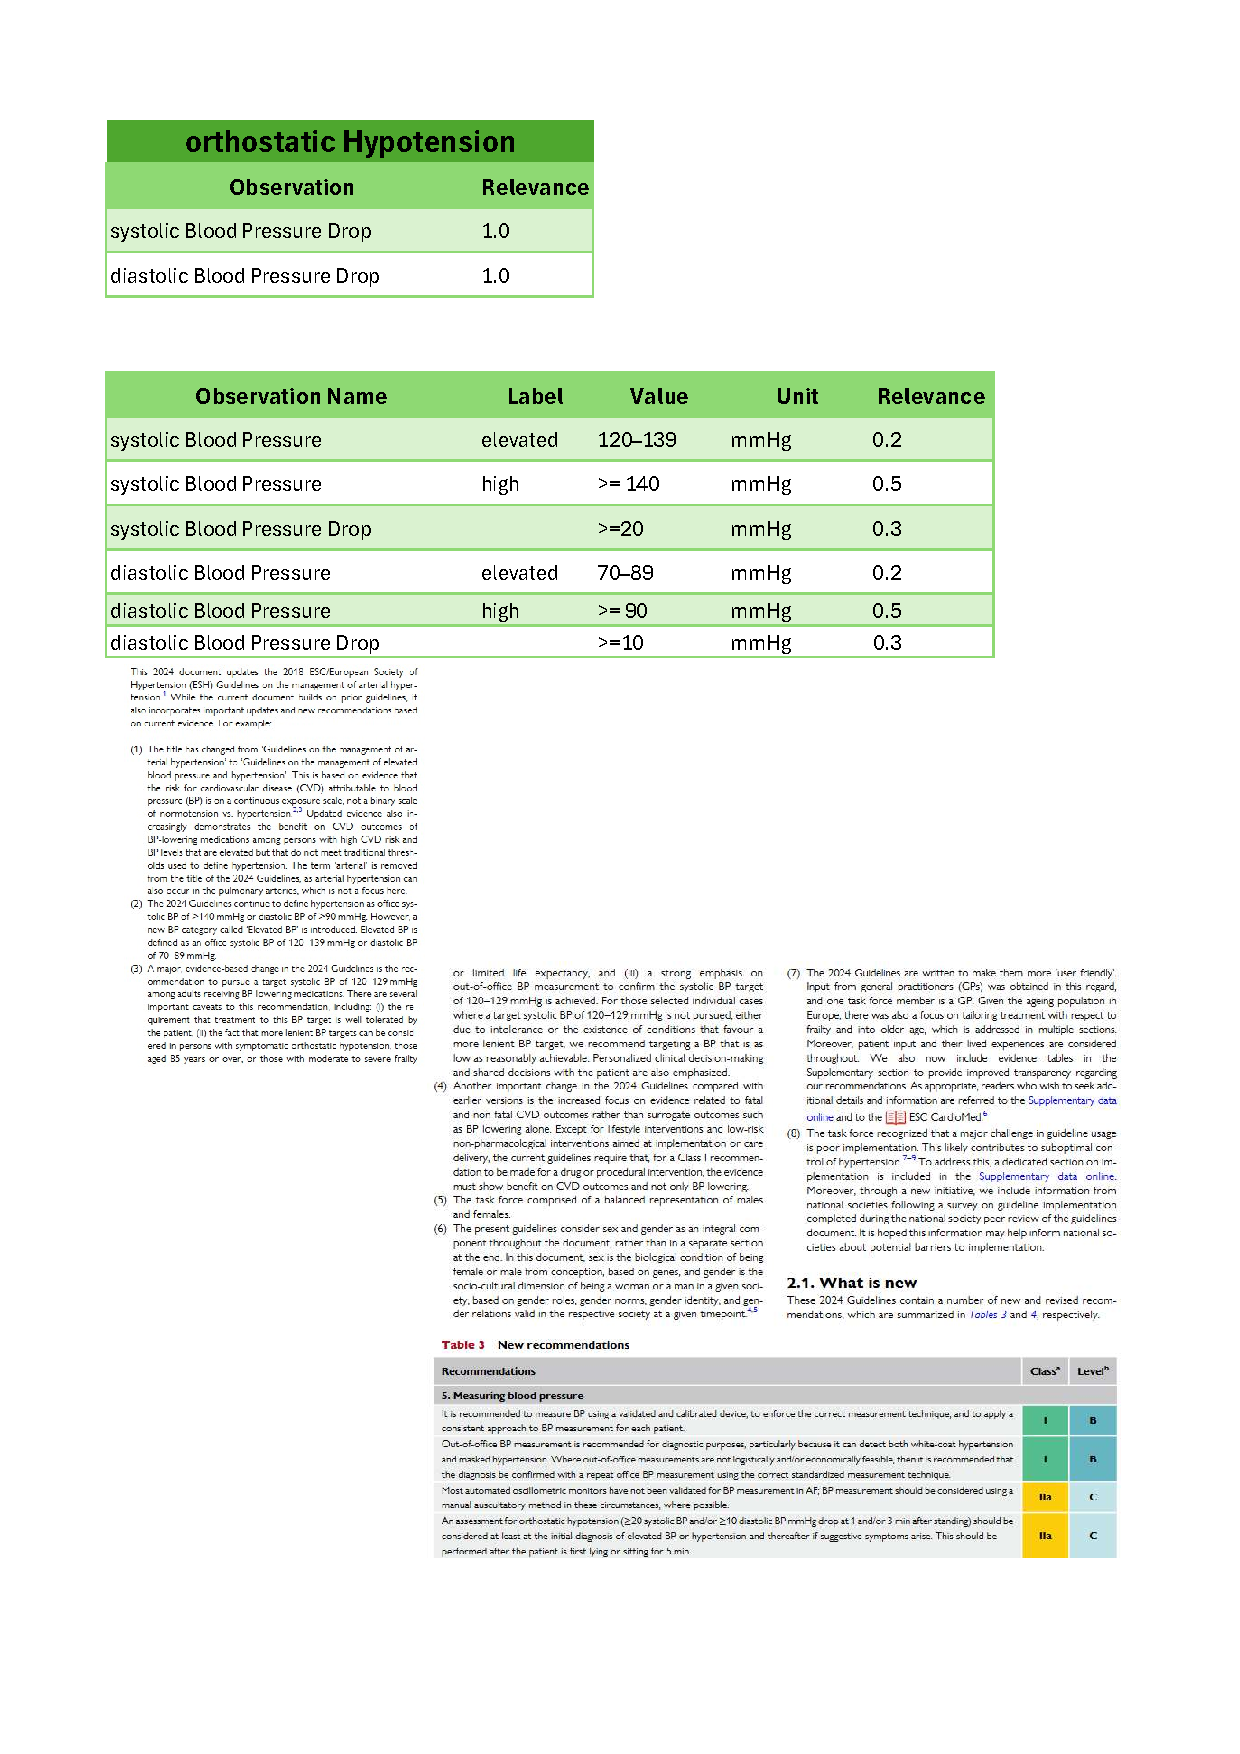
\includepdf[pages=-]{excel_2.pdf}
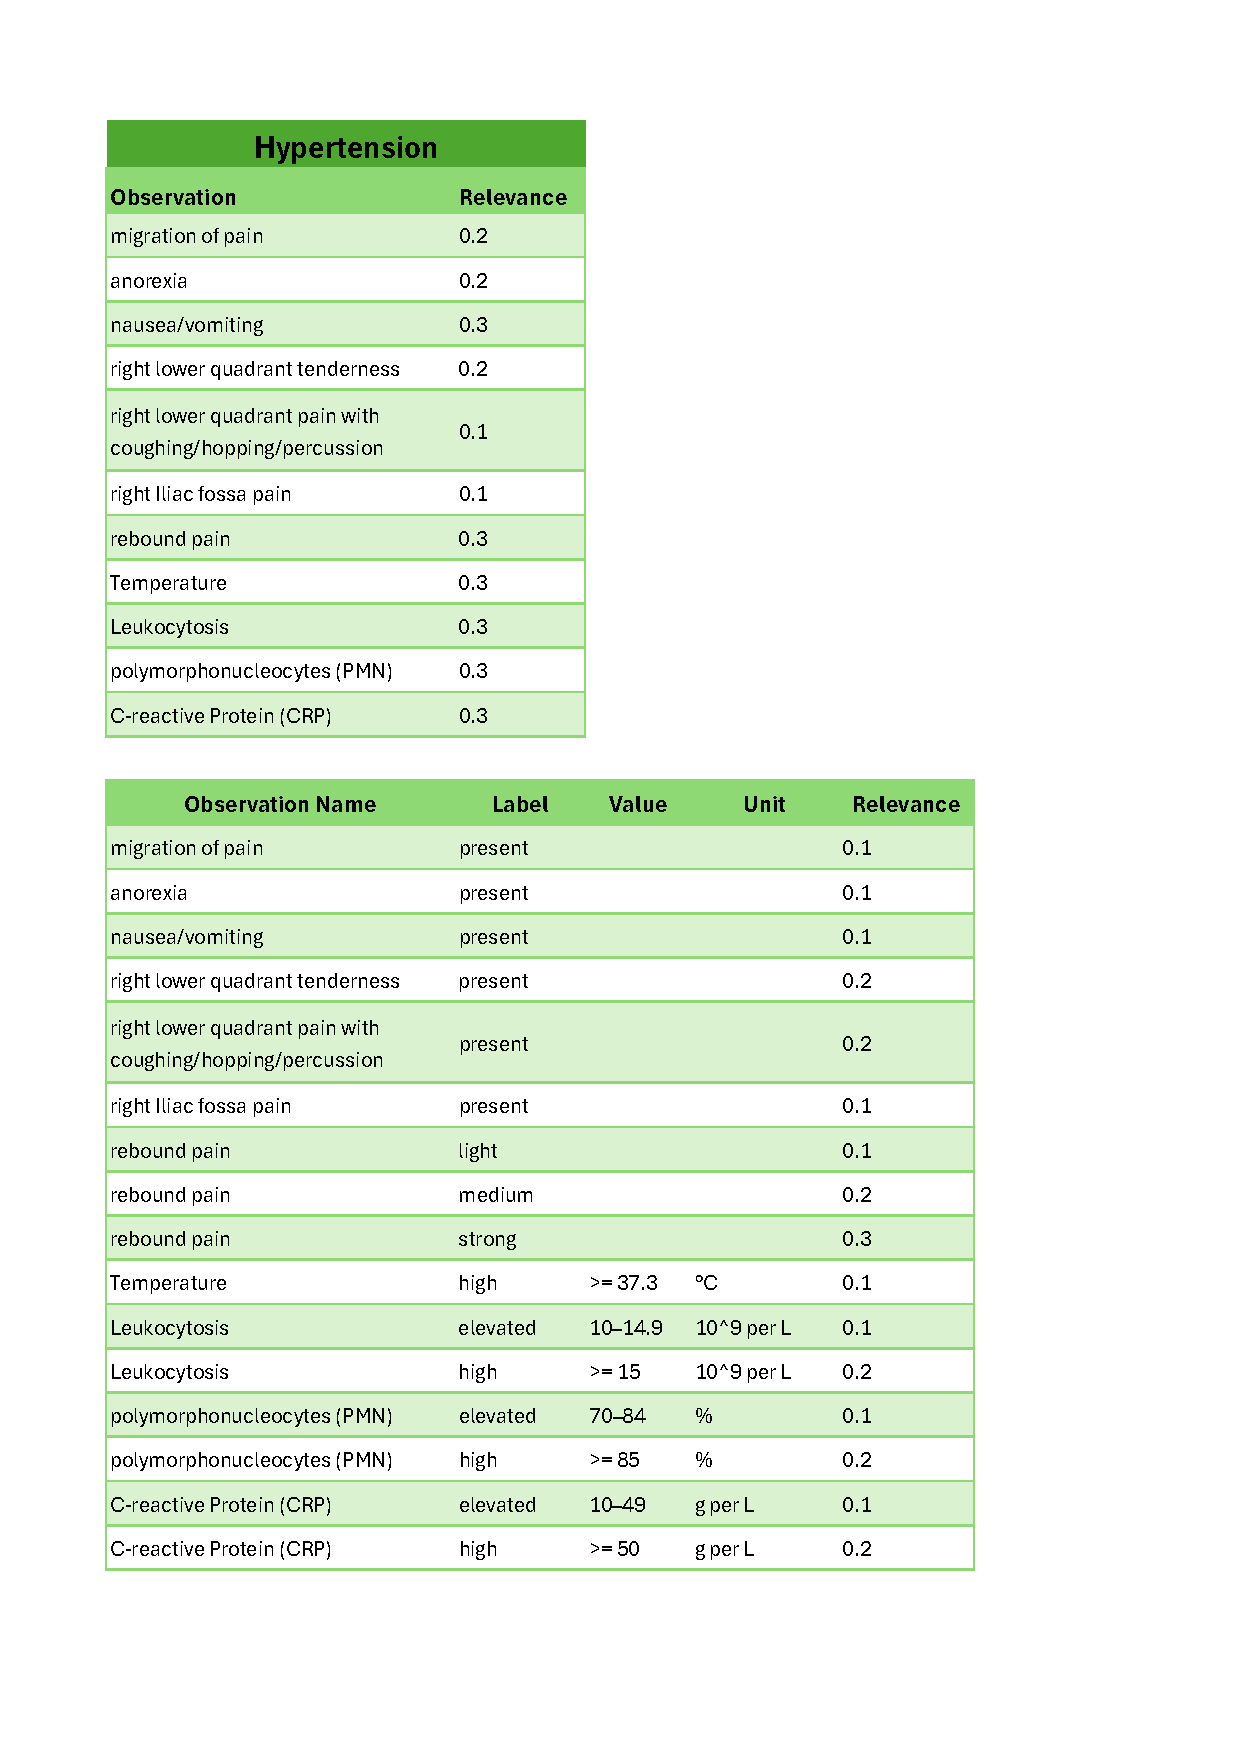
\includepdf[pages=-]{excel_3.pdf}

\subsection{Ground Truths}

\subsubsection*{Hypertension}


  \begin{minted}{json}
{
  "observations": [
    {
      "name": "systolic Blood Pressure",
      "context": [
        "Office"
      ],
      "patient_inferences": [
        {
          "gender": null,
          "age": null,
          "inferences": [
            {
              "label": "elevated",
              "value_criterion": {
                "value": [
                  120,
                  139
                ],
                "unit": "mmHg",
                "operator": null
              }
            },
            {
              "label": "high",
              "value_criterion": {
                "value": 140,
                "unit": "mmHg",
                "operator": ">="
              }
            }
          ]
        }
      ]
    },
    {
      "name": "diastolic Blood Pressure",
      "context": [
        "Office"
      ],
      "patient_inferences": [
        {
          "gender": null,
          "age": null,
          "inferences": [
            {
              "label": "elevated",
              "value_criterion": {
                "value": [
                  70,
                  89
                ],
                "unit": "mmHg",
                "operator": null
              }
            },
            {
              "label": "high",
              "value_criterion": {
                "value": 90,
                "unit": "mmHg",
                "operator": ">="
              }
            }
          ]
        }
      ]
    },
    {
      "name": "systolic Blood Pressure Drop",
      "context": [],
      "patient_inferences": [
        {
          "gender": null,
          "age": null,
          "inferences": [
            {
              "label": "large",
              "value_criterion": {
                "value": 20,
                "unit": "mmHg",
                "operator": ">="
              }
            }
          ]
        }
      ]
    },
    {
      "name": "diastolic Blood Pressure Drop",
      "context": [],
      "patient_inferences": [
        {
          "gender": null,
          "age": null,
          "inferences": [
            {
              "label": "large",
              "value_criterion": {
                "value": 10,
                "unit": "mmHg",
                "operator": ">="
              }
            }
          ]
        }
      ]
    }
  ],
  "conditions": [
    {
      "name": "hypertension",
      "observations": [
        "systolic Blood Pressure",
        "diastolic Blood Pressure"
      ]
    },
    {
      "name": "orthostatic hypotension",
      "observations": [
        "systolic Blood Pressure Drop",
        "diastolic Blood Pressure Drop"
      ]
    }
  ]
}
  \end{minted}
  \captionof{figure}{\textit{Ground Truth} for the Hypertension Guideline Text.\label{fig:GTHyp}}
  


\subsubsection*{Acute Appendicitis}

  \begin{minted}{json}
{
  "observations": [
    {
      "name": "migration of pain",
      "context": [],
      "patient_inferences": [
        {
          "gender": null,
          "age": null,
          "inferences": [
            {
              "label": "present",
              "value_criterion": null
            }
          ]
        }
      ]
    },
    {
      "name": "anorexia",
      "context": [],
      "patient_inferences": [
        {
          "gender": null,
          "age": null,
          "inferences": [
            {
              "label": "present",
              "value_criterion": null
            }
          ]
        }
      ]
    },
    {
      "name": "nausea/vomiting",
      "context": [],
      "patient_inferences": [
        {
          "gender": null,
          "age": null,
          "inferences": [
            {
              "label": "present",
              "value_criterion": null
            }
          ]
        }
      ]
    },
    {
      "name": "right lower quadrant tenderness",
      "context": [],
      "patient_inferences": [
        {
          "gender": null,
          "age": null,
          "inferences": [
            {
              "label": "present",
              "value_criterion": null
            }
          ]
        }
      ]
    },
    {
      "name": "right lower quadrant pain with coughing/hopping/percussion",
      "context": [],
      "patient_inferences": [
        {
          "gender": null,
          "age": null,
          "inferences": [
            {
              "label": "present",
              "value_criterion": null
            }
          ]
        }
      ]
    },
    {
      "name": "right Iliac fossa pain",
      "context": [],
      "patient_inferences": [
        {
          "gender": null,
          "age": null,
          "inferences": [
            {
              "label": "present",
              "value_criterion": null
            }
          ]
        }
      ]
    },
    {
      "name": "rebound pain",
      "context": [],
      "patient_inferences": [
        {
          "gender": null,
          "age": null,
          "inferences": [
            {
              "label": "light",
              "value_criterion": null
            },
            {
              "label": "medium",
              "value_criterion": null
            },
            {
              "label": "strong",
              "value_criterion": null
            }
          ]
        }
      ]
    },
    {
      "name": "Temperature",
      "context": [],
      "patient_inferences": [
        {
          "gender": null,
          "age": null,
          "inferences": [
            {
              "label": "high",
              "value_criterion": {
                "value": 37.3,
                "unit": "°C",
                "operator": ">="
              }
            }
          ]
        }
      ]
    },
    {
      "name": "Leukocytosis",
      "context": [],
      "patient_inferences": [
        {
          "gender": null,
          "age": null,
          "inferences": [
            {
              "label": "elevated",
              "value_criterion": {
                "value": [
                  10000,
                  14900
                ],
                "unit": "per $\mu$L",
                "operator": null
              }
            },
            {
              "label": "high",
              "value_criterion": {
                "value": 15000,
                "unit": "per $\mu$L",
                "operator": ">="
              }
            }
          ]
        }
      ]
    },
    {
      "name": "polymorphonucleocytes (PMN)",
      "context": [],
      "patient_inferences": [
        {
          "gender": null,
          "age": null,
          "inferences": [
            {
              "label": "elevated",
              "value_criterion": {
                "value": [
                  70,
                  84
                ],
                "unit": "%",
                "operator": null
              }
            },
            {
              "label": "high",
              "value_criterion": {
                "value": 85,
                "unit": "%",
                "operator": ">="
              }
            }
          ]
        }
      ]
    },
    {
      "name": "C-reactive Protein (CRP)",
      "context": [],
      "patient_inferences": [
        {
          "gender": null,
          "age": null,
          "inferences": [
            {
              "label": "elevated",
              "value_criterion": {
                "value": [
                  10,
                  49
                ],
                "unit": "g per L",
                "operator": null
              }
            },
            {
              "label": "high",
              "value_criterion": {
                "value": 50,
                "unit": "g per L",
                "operator": ">="
              }
            }
          ]
        }
      ]
    }
  ],
  "conditions": [
    {
      "name": "acute appendicitis",
      "observations": [
        "migration of pain",
        "anorexia",
        "nausea/vomiting",
        "right lower quadrant tenderness",
        "right lower quadrant pain with coughing/hopping/percussion",
        "right Iliac fossa pain",
        "rebound pain",
        "Temperature",
        "Leukocytosis",
        "polymorphonucleocytes (PMN)",
        "C-reactive Protein (CRP)"
      ]
    }
  ]
}
  \end{minted}
  \captionof{figure}{\textit{Ground Truth} for the Acute Appendicitis Text.\label{fig:GTAcu}}
  

\end{document}
